%
%  Created by Kasper Nybo Hansen on 2011-05-22.
%  Copyright (c) 2011 Kasper Nybo Hansen. All rights reserved.
%
%
\documentclass[10pt]{article}

\RequirePackage{nybohansenPreamble}

\newcommand{\authorName}{Kasper Nybo Hansen}
\newcommand{\authorEmail}{nybo@diku.dk}
\newcommand{\titleName}{Exam Notes}
\newcommand{\courseName}{Advanced Algorithms}

\author{\authorName \\\texttt{\small{\authorEmail}}}
\title{\textsc{\titleName \\ \courseName}}
% \date{}
\makeindex

\begin{document}

\maketitle 

\tableofcontents
\clearpage \newpage
\section{Max Flow} % (fold)
\label{sec:max_flow}

\subsection{Disposition Max Flow} % (fold)
\label{sub:disposition}

\begin{itemize}
  \item Draw directed graph
  \item Definition of flow
  \begin{itemize}
    \item Capacity constraint
    \item Flow conservation
  \end{itemize}
  \item Draw residual network
  \item Define cut - Partition graph into two etc.
  \begin{itemize}
    \item Define flow across cut
    \item Define capacity across cut
    \item Show Upper bound on flow equals capacity
  \end{itemize}
  \item Min-cut theorem
  \begin{itemize}
    \item f is a max flow  
    \item No augmenting paths
    \item There exist a cut with capacity equal to the flow value
    \begin{itemize}
      \item $1 \Leftrightarrow 2$ Contradiction
      \item $2 \Leftrightarrow 3$ Divide $G$ into two sets, $S$ and $T$, Where sets S contains nodes reachable from $S$ in $G_g$, and $T$ nodes not Reachable from $S$ in $G_f$. Show that the flow of the cut is equal to the capacity.
      \item $3 \Leftrightarrow 1$ Use that the capacity is a upper bound
    \end{itemize}
  \end{itemize}
  \item Ford-fulkerson and running time
  \item Edmonds Karp improving
\end{itemize}
% subsection disposition (end)Disposition

\newpage

The problem of max flow is finding a flow in a directed graph from a source to a sink. In the case of multiple sources and sinks, one can extend the graph by introducing a \emph{super source} and a \emph{super sink}.

\subsection{Definitions} % (fold)
\label{sub:definitions}
Let $G = (V,E)$ be a directed graph containing a source vertex $s \in V$ and sink vertex $t \in V$. Let every node $v \in V$ be reachable from $s$ and let $t$ be reachable from every node $v \in V$. Let each edge $(u,v) \quad \forall u,v \in V$ have a capacity $c(u,v) \geq 0$. The a flow is a real-valued function $f: V \times V \leftarrow R$, satisfying the capacity constraint and the flow conservation property. The capacity constraint says that the flow of an edge cannot exceed the capacity i.e
\begin{equation}
  0 \leq f(u,v) \leq c(u,v)
\end{equation} 
and the flow conservation property says that the total flow going into a vertex $u$ must be equal to the total flow going out of the vertex $u$, where $u \in V \setminus \{s,t\}$ i.e
\begin{equation}
  \sum_{v \in V} f(v,u) = \sum_{v \in V} f(u,v) \qquad u \in V \setminus \{s,t\}
\end{equation} 
The flow value, $|f|$, is calculated as
\begin{equation}
  |f| = \sum_{v \in V} f(s,v) - \sum_{v \in V} f(v,s)
\end{equation}
i.e. the flow value is calculated as the total flow going out of the source vertex minus the total flow going in.
% subsection definitions (end)

\subsection{Residual network} % (fold)
\label{sub:residual_network}
Let $f$ be a feasible flow in $G = (V,E)$. Let $G_f$ denote the residual network of $G$ induced by $f$, and let $f'$ be a flow in $G_f$. Then the function 
\begin{equation}
  (f \uparrow f')(u,v) = f(u,v)+f'(u,v)-f'(v,u) \qquad \forall (u,v) \in E
\end{equation}
denotes the augmentation of flow $f$ by flow $f'$.

It can be shown that $f \uparrow f'$ is a flow in $G$ and that the value is $|f \uparrow f'| = |f| + |f'|$.
% subsection residual_network (end)

\subsection{Cut} % (fold)
\label{sub:cut}
Given a graph $G = (V,E)$ a cut is a partitioning such that $V$ is divided into two subset $X$ and $Y$. We define the flow across a cut as
\begin{equation}
  f(X,Y) = \sum_{x \in X} \sum_{y \in Y} f(x,y) - \sum_{x \in X} \sum_{y \in Y} f(y,x)
\end{equation} 
thus the flow value of a cut is the total flow going from one subset to the other minus the total flow going the other way.

Let $G = (V,E)$, $X  = \subset V$, $Y = V \setminus X$, $s \in X$ and $t \in Y$. The partition $(X,Y)$ is then called a cut. The \emph{net flow} is defined as $f(X,Y)$. The capacity of the cut is defined as

\begin{equation}
 c(X,Y) = \sum_{u \in X, v \in Y} c(u,v)
\end{equation}
thus the capacity of a cut, is the total capacity of all connections between the two subsets.

% subsection cut (end)

\subsection{Min-cut theorem} % (fold)
\label{sub:min_cut_theorem}
A Min-cut is a cut where the capacity over all cuts is minimized. We thus choose to partition the $V$ such that the capacity, $c(X,Y)$, between the two sets are minimized.

Show that an augmenting path increases the flow value. This is intuitively true, since when finding an augmenting path, it is added to the original graph.

Show that the flow value has an upper bound. Let $V$, in a graph $G = (V,E)$, be partitioned into two subsets, $S$ and $T$. The flow value then has a upper bound equal to the capacity of the cut. The following proves this statement
\begin{align*}
 |f| &= f(S,T)  \\ 
     &= \sum_{s \in S} \sum_{t \in T} f(s,t) - \sum_{s \in S} \sum_{t \in T} f(t,s) \\
     &\leq \sum_{s \in S} \sum_{t \in T} f(s,t) \\
     &\leq \sum_{s \in S} \sum_{t \in T} c(s,t) \\
     &= c(S,T)
\end{align*}


\begin{theorem}

  Given a graph $G = (V,E)$ and a flow $f$ ($f$ does not necessarily be a max flow), the min-cut theorem states that the following three statements are equivalent

  \begin{enumerate}
    \item $f$ is a maximum flow in G, i.e the flow value, $|f|$, is maximized
    \item There are no augmenting paths in the residual network, $G_f$
    \item $|f| = c(S,T)$ for some cut $(S,T)$ in $G$
  \end{enumerate}
  
\end{theorem}

\begin{proof}

The proof is done in a circular fashion. We will start by showing $1 \Rightarrow 2$ by contradiction.   
  
Let $f$ be a maximum flow in $G$. Let there be an augmenting path in the residual network. Hence there is a nonzero flow $f'$ in $G_f$. Thus $f \uparrow f'$ is strictly greater than $f$. This is a contradiction compared to our initial belief that $f$ was a maximum.
\end{proof} 

We will now show $2 \Rightarrow 3$
\begin{proof}
Assume that there are no augmenting paths in $G_f$, i.e. there are no paths between $s$ and $t$ in $G_f$, and they are there disconnected. Now partition $G$ into two subsets, $S$ and $T$, such that $S = \{v \in V: \text{There is a path from $s$ to $v$ in $G_f$}\}$ and $T = V\setminus S$. I.e. $S$ contains the vertices reachable from the source node $s$ in $G_f$. Then $(S,T)$ is a cut. We now want to show that the value of this cut is equal to $|f|$. 

Let $u \in S$ and $v \in T$. 

If the edge $(u,v) \in E$, i.e. $(u,v)$ is an edge going from $S$ to $T$, then the flow going through this edge must be equal to the capacity, i.e. $f(u,v) = c(u,v)$ otherwise $(u,v) \in E_f$ which would place $v$ in set $S$. 

If the edge $(v,u) \in E$, i.e. $(v,u)$ is an edge going from the $T$ to $S$, then we must have that $f(v,u)=0$, otherwise $c_f(u,v) = f(v,u)$ would be positive and therefore $(u,v) \in E_f$ which would place $v$ in set $S$.

Thus the flow of the cut is

\begin{align*}
 f(S,T) &= \sum_{u \in S} \sum_{v \in T} f(u,v) - \sum_{u \in S} \sum_{v \in T} f(v,u) \\
        &= \sum_{u \in S} \sum_{v \in T} f(u,v) - 0 \\ 
        &= c(S,T) 
\end{align*}
\end{proof} 


The final thing we need to show is $3 \Rightarrow 1$. We thus need to show that $|f| = c(S,T)$ implies that $|f|$ is maximized. 

\begin{proof}
  We have shown that a flow has a upper bound of $c(S,T)$ i.e. $|f| \leq c(S,T)$. This means that $|f|$ must be maximized when $|f| = c(S,T)$.  
\end{proof}

The min-cut is the dual of the max flow.
% subsection min_cut_theorem (end)
                                                          
\subsection{Ford-Fulkerson and Edmonds Karp} % (fold)
\label{sub:ford_fulkerson_and_edmonds_karp}
The Ford-Fulkerson method works as follows:
\begin{verbatim}
  Initialize all edges to have a 0 flow
  Construct the residual network G_f   
  while augmenting paths exists in G_f do
    Find an augmenting path in G_f
    augment f with the max value found in the augmenting path 
    Construct the residual network for the increased flow
  loop 
\end{verbatim}

An example of running the Ford-Fulkerson method can be seen on figure \ref{fig1}

\begin{figure}[ht]
\centering
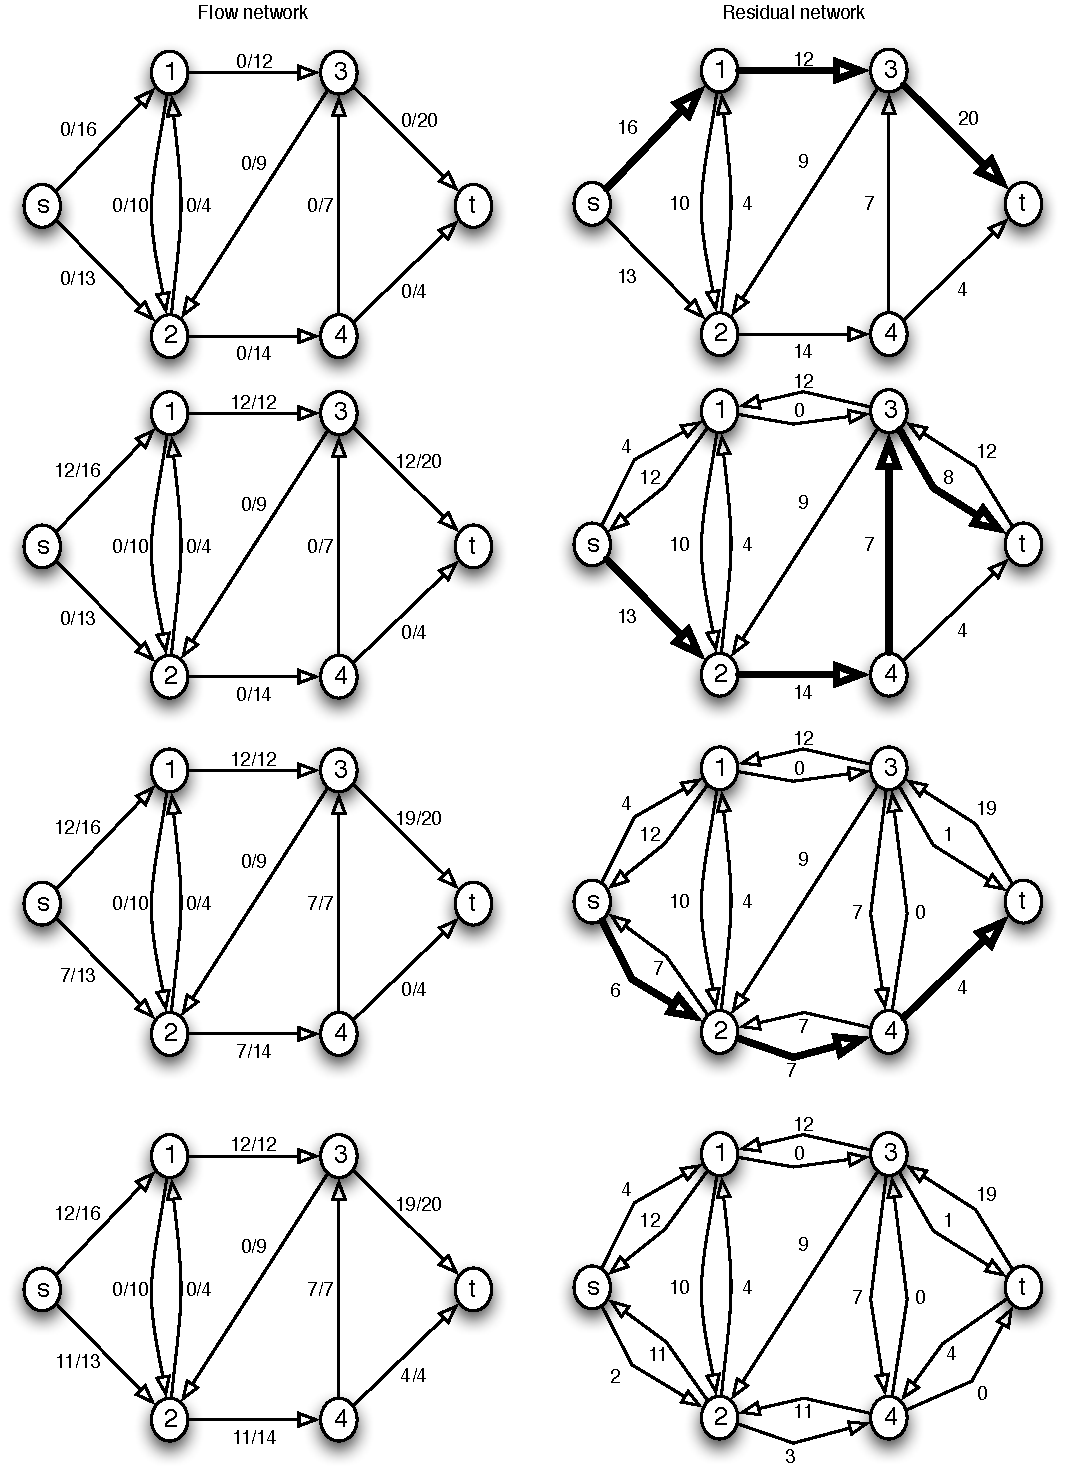
\includegraphics[width=0.9\textwidth]{figures/fig1.pdf}
\caption{Example of running the Ford-Fulkerson method. Left side is the flow network, right side is the residual network, with bold lines representing augmenting paths.}
\label{fig1}
\end{figure}

The running time of the Ford-Fulkerson can be expressed as $\O(E\dot f*)$ where $f*$ denotes the value of the max flow. At each iteration we search through $\O(E)$ edges, and the maximum number of iterations is $f*$. An illustration of this running time can be seen in figure \ref{fig2}.

\begin{figure}[ht]
\centering
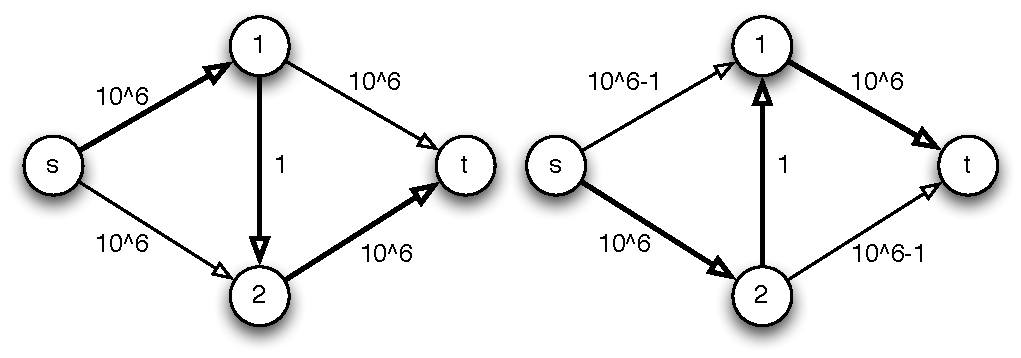
\includegraphics[width=0.9\textwidth]{figures/fig2.pdf}
\caption{Illustration of the complexity of the Ford-Fulkerson algorithm}
\label{fig2}
\end{figure}

This running time can be improved by selecting the augmenting path by breath first. Breath first chooses the shortest path with capacity between the source and sink. This is exactly what Edmonds-Karp does, thus Edmonds-Karp is a specialized version of the Ford-Fulkerson method. The running time of Edmonds-Karp is $\O(V^2E)$.


% subsection ford_fulkerson_and_edmonds_karp (end)

% section max_flow (end)
\clearpage \newpage
\section{Linear Programming} % (fold)
\label{sec:linear_programming}

\subsection{Disposition Linear Programming} % (fold)
\label{sub:disposition2}
\begin{itemize}
  \item Show small problem, draw graph
  \item Standard form, and slack form
  \item SIMPLEX algorithm, that moves along edges, needs initial solution e.g. try $0$
  \item Some cases $0$ doesn't work, form auxiliary program $-x_0$. Add $-x_0$ to all constraints
  \item It maximizes the objective function by making it better until all coefficients are $0$.
  \item It does this by pivoting, basis is left side of slack, non basic is right.
  \item Explain simplex by Flow diagram
  \item Show the dual, I.e. $b's$ up into objective function, transpose $a$ and $c$ into right-hand side constraints
  \item Weak duality
  \begin{equation}
    \sum_{j=1}^n c_jx_j \leq \sum{j_1}^m b_iy_i
  \end{equation}
  \item A solution, $\bar{x}$ to the primal, is also a solution to the dual. 
  \begin{equation} 
  \bar{y}_i = 
  \left\{
  \begin{array}{rl} 
    -c'_{n+i} & if (n+1) \in N \\
    0 &  
  \end{array} 
  \right. 
  \end{equation} 
  Need to show 2 things
  \begin{itemize}
    \item Need to show that $\bar{y}_i$ is a feasible solution to the dual
    \item $\sum_{j=1}^n c_j\bar{x}_j = \sum_{j=1}^m c_j\bar{y}_j$
  \end{itemize}
\end{itemize}
% subsection disposition (end)
\newpage
In linear programming we want to maximize (or minimize) a linear function, under a number of constraints. An example of a linear program is
\begin{align}
 \max &\quad x_1 + x_2 \label{linprop1}\\ 
 \text{St.} &\quad  4x_1 - x_2  \leq 8 \nonumber\\
            &\quad  2x_1 + x_2  \leq 10 \nonumber\\
            &\quad  5x_1 - 2x_2 \leq -2 \nonumber\\            
            &\quad  x_1,x_2,x_3 \geq 0  \nonumber
\end{align}
\ref{linprop1} is called the objective function.
                                                                      
A linear program in 2 dimensions can be illustrated as figure \ref{fig3}. The gray area is called the feasible region.
\begin{figure}[ht]
\centering
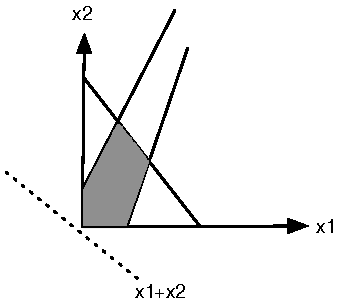
\includegraphics[width=0.5\textwidth]{figures/fig3.pdf}
\caption{Illustration of a simple linear program where the objective function is $x_1 + x_2$. The feasible region is gray.}
\label{fig3}
\end{figure}

A linear program can be written in two ways. Standard form and slack form. When a linear program is written in standard form it takes the following form
\begin{align*}
\max &\quad \sum_{j=1}^n c_jx_j  \\ 
 \text{S.t.} &\quad \sum_{j=1}^n a_{ij}x_j \leq b_i \qquad i=1,2,\ldots,m\\
             &\quad x_j \geq 0 \qquad i=1,2,\ldots,n\\
\end{align*}
where $m$ is the number of constraints and $n$ is the number of variables. One could think of $a$ as a matrix having, $m$ rows and $a$ columns. Every linear program can be rewritten to slack form. 

\subsection{Converting into standard form} % (fold)
\label{sub:converting_into_standard_form}
A linear program does not have to take standard form. But we can always turn a linear program into standard form. The following section describes how to convert a non-standard form linear program into standard form.

\begin{itemize}
  \item If the program is a minimization problem, then it can be turned into a maximization problem by multiplying the objective function by -1. The constraints are not changed, since the feasible region is the same, regardless if we want to maximize or minimize an objective function under the same constraints.                                                                         
  \item If the linear program contains variables, $x_j$ without nonnegative constraints we can replace $x_j$ so $x_j = x_j'-x_j''$, and add the constraints $x_j', x_j''>0$.
  \item If the linear program contains equality constraints, then replace each equality with to inequality constraints going opposite ways, i.e $a = b \Leftrightarrow a \leq b \wedge a \geq b$. 
  \item If the linear program contains inequality constraints, but instead of less than, they are greater than, then multiply the constraint with $-1$.
\end{itemize}

The following is an example of how to convert a non-linear program into standard form. 
\begin{align*}
 \min &\quad -2x_1 + 3x_2  \\ 
 \text{St.} &\quad  x_1 + x_2  = 7 \\
            &\quad  x_1 - 2x_2 \leq 4 \\
            &\quad  x_1        \geq 0  
\end{align*}

Start by making it a maximization problem, i.e. multiply the objective function with $-1$.
\begin{align*}
 \max &\quad 2x_1 - 3x_2  \\ 
 \text{St.} &\quad  x_1 + x_2  = 7 \\
            &\quad  x_1 - 2x_2 \leq 4 \\
            &\quad  x_1        \geq 0  
\end{align*}
Next place $x_2$ under the nonnegative constraint. Let $x_2 = x_2'-x_2''$ then
\begin{align*}
 \max &\quad 2x_1 - 3x_2' +3x_2''  \\ 
 \text{St.} &\quad  x_1 + x_2'-x_2''  = 7 \\
            &\quad  x_1 - 2x_2' +2x_2'' \leq 4 \\
            &\quad  x_1, x_2', x_2''    \geq 0  
\end{align*}
Make a cleanup so we remove those pesky primes, just rename $x_2' = x_2$ and $x_2'' = x_3$.
\begin{align*}
 \max &\quad 2x_1 - 3x_2 +3x_3  \\ 
 \text{St.} &\quad  x_1 + x_2-x_3  = 7 \\
            &\quad  x_1 - 2x_2 +2x_3 \leq 4 \\
            &\quad  x_1, x_2, x_3    \geq 0  
\end{align*}
Lets remove the equality sign, by replacing the equality with to opposite directed inequalities i.e.
\begin{align*}
 \max &\quad 2x_1 - 3x_2 +3x_3  \\ 
 \text{St.} &\quad  x_1 + x_2-x_3  \leq 7 \\
            &\quad  x_1 + x_2-x_3  \geq 7 \\
            &\quad  x_1 - 2x_2 +2x_3 \leq 4 \\
            &\quad  x_1, x_2, x_3    \geq 0  
\end{align*}
Final thing we need to do, is to turn the greater than into a less than my multiplying with $-1$, i.e.
\begin{align}
 \max &\quad 2x_1 - 3x_2 +3x_3  \label{linprop2}\\ 
 \text{St.} &\quad  x_1 + x_2-x_3  \leq 7 \nonumber\\
            &\quad  -x_1 - x_2 + x_3  \leq -7 \nonumber\\
            &\quad  x_1 - 2x_2 +2x_3 \leq 4 \nonumber\\
            &\quad  x_1, x_2, x_3    \geq 0  
\end{align}
and the linear program in now in standard form.
% subsection converting_into_standard_form (end)


\subsection{Slack form} % (fold)
\label{sub:slack_form}
In slack form, the inequalities are replaced by equalities and a number of slack variables are introduced. We can rewrite the standard form linear program shown in \ref{linprop2} to slack form as
\begin{align*}
 \max &\quad 2x_1 - 3x_2 +3x_3 \\ 
 \text{St.} &\quad  x_4 = 7 - x_1 - x_2 + x_3\\
            &\quad  x_5 = -7 + x_1 + x_2 -x_3\\
            &\quad  x_6 = 4 -x_1 + 2x_2 -2x_3\\
            &\quad  x_1, x_2, x_3, x_4, x_5, x_6    \geq 0  
\end{align*}
We have just introduced the three \emph{basic variables} $x_4,x_5,x_6$ and rearranged the original non-basic variables. In general when going from standard to slack form, you need $m$ new slack variables, where $m$ denotes the number of constraints.
% subsection slack_form (end)

\subsection{SIMPLEX algorithm} % (fold)
\label{sub:simplex_algorithm}
There exists several methods to solve linear programs. Some methods are polynomial, but doesn't work well in practice. A non polynomial method is called simplex. Simplex has it name from the shape of the feasible region.

The geometric interpretation of SIMPLEX is as follows. It starts at a corner point: the origin, and looks at the edges incident with that point. Then it chooses one, and moves along an edge which makes the objective value get larger (or stay the same). If the edge goes on forever, then the LP is unbounded; if the edge does not go on forever, it ends up at another corner point. Then the Simplex Method does the same thing over and over again, until it stops at a certain point. That point is the place where the objective value is the largest.


Normally, this would only lead you to a local maximum, instead of the global maximum, but this cannot happen when solving a LP. This is because the objective values and inequalities are linear in form.

Given a linear program

\begin{align}
  \max &\quad 2x_1 - x_2 \label{aux1}\\ 
  \text{St.} &\quad  2x_1 - x_2  \leq 7 \nonumber\\
             &\quad  x_1 - 5x_2  \leq -7 \nonumber\\
             &\quad  x_1, x_2    \geq 0 
\end{align}

Simplex needs the problem in standard form, it starts by converting the problem into slack form, i.e.
\begin{align}
  z  &= 2x_1 - x_2 \label{aux2}\\ 
  x_3 &= 7 - 2x_1 + x_2 \nonumber\\
  x_4 &= -7-x_1 + 5x_2  \nonumber\\
  &x_1, x_2, x_3, x_4    \geq 0 
\end{align}


it then finds a initial solution. Typically this solution is found by setting the variables to $0$. Sometimes the initial solution isn't feasible as can be see in \ref{aux2}. In this case, we need to formulate an auxiliary program. The auxiliary program for \ref{aux1} is

\begin{align}
  \max &\quad -x_0 \\ 
  \text{St.} &\quad  2x_1 - x_2 -x_0 \leq 2 \nonumber\\
             &\quad  x_1 - 5x_2 -x_0 \leq -4 \nonumber\\
             &\quad  x_1, x_2,x_0    \geq 0 \nonumber 
\end{align}
 
The auxiliary program is then solved with the SIMPLEX algorithm. It starts by rewriting the problem into slack form
\begin{align}
    z &= -x_0 \\ 
  x_3 &= 2 - 2x_1 + x_2 + x_0  \nonumber\\
  x_4 &= -4 - x_1  + 5x_2 + x_0  \nonumber\\
  &x_0, x_1, x_2, x_3, x_4    \geq 0 \nonumber 
\end{align}
And pivot's, so $x_0$ enters the basis, on the constraint that is most negative
\begin{align}
    z &= -x_0 \\ 
  x_3 &= 2 - 2x_1 + x_2 + x_0  \nonumber\\
  x_0 &= 4 + x_1 -5x_2 + x_4    \nonumber\\
  &x_0, x_1, x_2, x_3, x_4    \geq 0 \nonumber 
\end{align}
and substitutes $x_0$ into the objective function and the constraints
\begin{align}
    z &= -4 - x_1 + 5x_2 - x_4\\ 
  x_0 &= 4 + x_1 - 5x_2 + x_4   \nonumber\\
  x_3 &= 6 - x_1 - 4x_2 + x_4   \nonumber\\
  &x_0, x_1, x_2, x_3, x_4    \geq 0 \nonumber 
\end{align}
The basic feasible solution to this problem is $(x_0, x_1, x_2, x_3, x_4) = (4, 0, 0, 6, 9)$. We want the optimal solution so we need to do a pivot. Since $5x_2$ is the only one that is nonnegative, we investigate this: $x_0$ binds with $4/5=16/20$, and $x_3$ binds with $6/4=30/20$. We thus choose to pivot on $x_0$ and $x_2$, since $x_0$ is the most binding.
\begin{align}
    z &= -4 - x_1 + 5(\frac{4}{5} - \frac{1}{5} x_0 + \frac{1}{5} x_1 + \frac{1}{5} x_4) - x_4\\ 
  x_2 &= \frac{4}{5} - \frac{1}{5} x_0 + \frac{1}{5} x_1 + \frac{1}{5} x_4    \nonumber\\
  x_3 &= 6 - x_1 - 4(\frac{4}{5} - \frac{1}{5} x_0 + \frac{1}{5} x_1 + \frac{1}{5} x_4) + x_4   \nonumber\\
  &x_0, x_1, x_2, x_3, x_4    \geq 0 \nonumber 
\end{align}
reducing yields
\begin{align}
    z &= - x_0 \label{aux3}\\ 
  x_2 &= \frac{4}{5} - \frac{1}{5} x_0 + \frac{1}{5} x_1 + \frac{1}{5} x_4    \nonumber\\
  x_3 &= \frac{14}{5} + \frac{4}{5} x_0 - \frac{9}{5} x_1 + \frac{1}{5} x_4    \nonumber\\
  &x_0, x_1, x_2, x_3, x_4    \geq 0 \nonumber 
\end{align}
this slack form is the final solution to the auxiliary problem. Since $x_0 = 0$ we know it's optimal, and that the initial problem was feasible. Since $x_0=0$ we can remove it from the set of constraints. The original objective function \ref{aux2} can then be restored, substituting the basic variables from \ref{aux1}, and retaining the constraints form \ref{aux3}

\begin{align}
    z &= - \frac{4}{5} + \frac{9}{5} x_1 - \frac{1}{5} x_4\\ 
  x_2 &= \frac{4}{5} + \frac{1}{5} x_1 + \frac{1}{5} x_4    \nonumber\\
  x_3 &= \frac{14}{5} - \frac{9}{5} x_1 + \frac{1}{5} x_4    \nonumber\\
  &x_1, x_2, x_3, x_4    \geq 0 \nonumber 
\end{align}

Setting this slack form to zero, yields the basic solution $(x_1, x_2, x_3, x_4) = (0, \frac{4}{5} , \frac{14}{5} , 0)$. This slack form can now be solved by using the SIMPLEX algorithm again.

a flow chart of the simplex can be seen in figure \ref{fig4}

\begin{figure}[ht]
\centering
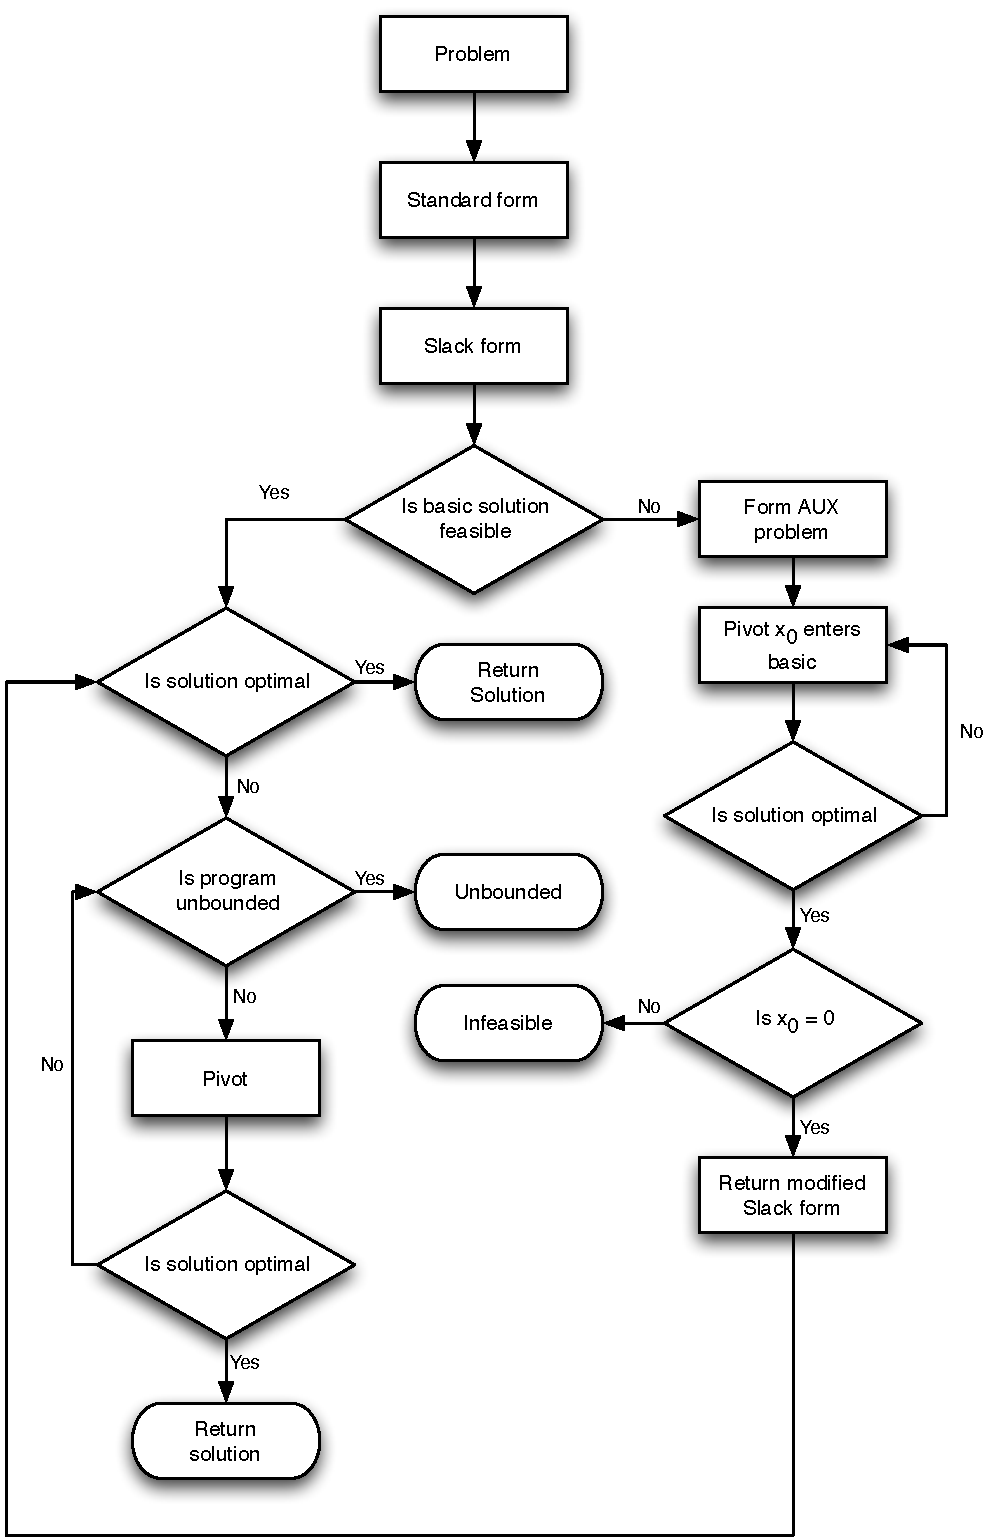
\includegraphics[width=0.9\textwidth]{figures/fig4.pdf}
\caption{Flowchart of the SIMPLEX algorithm}
\label{fig4}
\end{figure}

\subsubsection{Cycling} % (fold)
\label{ssub:cycling}
There is a risk that SIMPLEX cycles. This means that we at some point arrive at the same slack state as we have visited before. Cycling can be avoided by always choosing the entering variable with the smallest index, and furthermore if there are multiple exiting variables, always choose the one with the lowest index.
% subsubsection cycling (end)

% subsection simplex_algorithm (end)

\subsection{Duality} % (fold)
\label{sub:duality}

Duality means that finding a solution in one problem 

Given a linear program with $n$ variables and $m$ constraints
\begin{align}
 \max &\quad \sum_{j=1}^n c_jx_j  \nonumber\\ 
 \text{S.t.} &\quad \sum_{j=1}^n a_{ij}x_j \leq b_i \qquad i=1,2,\ldots,m\label{dual10}\\
             &\quad x_j \geq 0 \qquad i=1,2,\ldots,n \nonumber
\end{align}
and call this the \emph{primal}. We define the \emph{dual} as 
\begin{align}
 \min &\quad \sum_{i=1}^m b_iy_i  \nonumber\\ 
 \text{S.t.} &\quad \sum_{j=1}^m a_{ij}y_i \geq c_j \qquad j=1,2,\ldots,n \label{dual0}\\
             &\quad y_j \geq 0 \qquad i=1,2,\ldots,m \nonumber
\end{align}
The dual is a minimization problem and it has $m$ variables and $n$ constraints. Furthermore the less-than-equal-to has been replaced by greater-than-equal-to. Each $b_i$ in the primal is now part of the objective function as a coefficient. Each $c_j$ in the primal is now the right hand side of the constraints. If $a$ was a matrix then in the dual it is transposed. 

Example: Let the primal be
\begin{align}
 \max &\quad 3x_1 + x_2 + 2x_3\label{dual1}\\ 
 \text{St.} &\quad  x_1  + x_2  + 3x_3 \leq 30 \nonumber\\
            &\quad  2x_1 + 2x_2 + 5x_3 \leq 24 \nonumber\\
            &\quad  4x_1 + x_2  + 2x_3 \leq 36 \nonumber\\            
            &\quad  x_1,x_2,x_3 \geq 0  \nonumber
\end{align}
then the dual is
\begin{align}
 \min &\quad 30y_1 + 24y_2 + 36y_3 \label{dual2}\\ 
 \text{St.} &\quad  y_1 + 2y_2  + 4y_3  \geq 3 \nonumber\\
            &\quad  y_1 + 2y_2  + 1y_3  \geq 1 \nonumber\\
            &\quad  3y_1 + 5y_2  + 2y_3 \geq 2 \nonumber\\            
            &\quad  y_1, y_2, y_3 \geq 0  \nonumber
\end{align}

Weak linear-programming duality states the following
\begin{theorem}
  Given a feasible solution to the primal problem, $\bar{x}$, and a feasible solution to the dual problem, $\bar{y}$, then
  \begin{equation}
  \sum_{j=1}^n c_jx_j \leq \sum_{i=1}^m b_iy_i
  \end{equation}  
\end{theorem}
said in words: the primal is bounded above by the dual.

\begin{proof}
Let $\bar{x}$ and $\bar{y}$, be feasible solutions to the primal and the dual respectively.

From \ref{dual0} we know that $\sum_{j=1}^m a_{ij}y_i \geq c_j$. Thus we can write
\begin{equation}
\sum_{j=1}^n c_j\bar{x}_j \leq  \sum_{j=1}^n \left (\sum_{j=1}^m a_{ij}\bar{y}_i\right)\bar{x}_j   
\end{equation}
exchanging $\bar{x}_i$ and $\bar{y}_i$ yields
\begin{equation}
\sum_{j=1}^n c_j\bar{x}_j \leq  \sum_{j=1}^n \left (\sum_{j=1}^m a_{ij}\bar{x}_j\right)\bar{y}_i
\end{equation}
and \ref{dual10} gives us $\sum_{j=1}^m a_{ij}x_j \leq b_i$ which we can insert
\begin{equation}
\sum_{j=1}^n c_j\bar{x}_j \leq  \sum_{j=1}^m b_i\bar{y}_i
\end{equation}
and we arrive what we wanted to prove.
\end{proof}

The duality theorem states that if a feasible solution of the primal, is equal to a feasible solution to the dual, the this feasible solution is optimal to both the primal and the dual. More precisely the theorem states

\begin{theorem}
Let SIMPLEX terminate with a feasible basic solution $\bar{x}*=(x_1*,x_2*,\ldots,x_n*)$, and let $N$ denote the nonbasic and $B$ the basic variables for the final slack form. Let $c'$ denote the coefficients of the objective function in the final slack form. 

Now let $\bar{y}* = (y_1*,y_2,\ldots,y_m)$ be defined as

\begin{equation} 
\bar{y}* = 
\left\{
\begin{array}{rl} 
  -c'_{n+i} & \text{if } (n+i) \in N \\
   0 & \text{otherwise}
\end{array} 
\right. 
\end{equation} 

then $\bar{x}*$ is an optimal solution to the primal, and $\bar{y}*$ is an optimal solution to the dual and
\begin{equation}
  \sum_{j=1}^n c_jx_j* = \sum_{i=1}^m b_iy_i*
\end{equation}
\end{theorem}

\begin{proof}
In order to prove the above, we have to show that $\bar{y*}$ is a feasible solution to the dual, and that 
\begin{equation}
  \sum_{j=1}^n c_jx_j* = \sum_{i=1}^m b_iy_i*  
\end{equation}
\end{proof}
 
% subsection duality (end)

% section linear_programming (end)

\clearpage \newpage
\section{NP-completeness} % (fold)
\label{sec:np_completeness}

\subsection{Disposition NP-completeness} % (fold)
\label{sub:disposition_np_completeness}
\begin{itemize}
  \item What are hard problems, Problems that cannot be solved in polynomial time
  \item What is a language <- Describing instance of a problem so it can be answered with yes/no
  \begin{equation}
  HAM-CYCLE = \{\langle G \rangle: G \text{ is a hamilton cycle}\}   
  \end{equation}
  \item Reduction algorithm
  \begin{itemize}
    \item We can reduce one problem into another problem
    \item Must be done in polynomial time
    \item Answers from the original and reduced problem must be the same
  \end{itemize}
  \item Definition of P 
  \begin{equation}
    P = \{\text{L: L is accepted be a polynomial-time algorithm}\}
  \end{equation}
  \item Definition of NP
  \begin{equation}
    NP = \{\text{L: There exists an A, such that L is verified in polynomial time}\}
  \end{equation}
  \item Definition of NP-Complete
  \item Draw set, and explain what it would mean if $P = NP$.
  \begin{enumerate}
    \item $L \in NP$
    \item $L' \leq_p L \qquad \forall L' \in NP$
  \end{enumerate} 
  \item Show TSP is a NP-complete problem: $HAM-CYCLE \leq_p TSP$. Show two things
  \begin{itemize}
    \item Decision problem in NP (Verification in polynomial time)
    \item $HAM-CYCLE$ instance $G = (V,E)$, form complete graph $G' = (V,E')$ with
    \begin{equation} 
    e_i = 
    \left\{
    \begin{array}{rl} 
       0 &  e_i \in E\\
       1 &  otherwise
    \end{array} 
    \right. 
    \end{equation} 
  \end{itemize}
  Suppose $G$ has hamilton cycle $h$. Each edge resides in $G$ thus having cost 0 in $G'$. Suppose $G'$ has a tour $h'$ of cost 0. Then this tour can only occur if $h'$ is a hamilton cycle in $G$. 
\end{itemize}
% subsection disposition_np_completeness (end)
\newpage

NP-complete problems is a class of problems that has algorithms that run in \emph{super polynomial} time, i.e. there running time is thus $>\O(N^k)$, for some constant $k$.

NP-completeness only applies to decision problems. A optimization problem can easily be made into a decision problem by setting a bound. E.g. a shortest path problem\footnote{Finding the shortest path between two nodes in a graph} can be made into a decision problem, by asking: Is there a shortest path between these two nodes with at most length $k$?.  

When we are proving something is NP-complete, and therefore hard to solve, we are proving it under the constraint that no polynomial algorithm exist for a NP-complete problem. This assumption is still not proved formally (But if this does not hold, we have a BIG problem!).


\subsection{Language} % (fold)
\label{sub:language}
A language describes a problem. E.g. the language for the Hamilton cycle problem can be described as "Does the graph $G$ have a Hamilton cycle", or more formally
\begin{equation}
HAM-CYCLE = \{\langle G \rangle: G \text{ is a hamilton cycle}\}   
\end{equation}
The contents between the $\langle$ and $\rangle$ is the input to the problem.
% subsection language (end)

\subsection{Reduction algorithm} % (fold)
\label{sub:reduction_algorithm}
Suppose we have a decision problem $A$ that we want to solve in polynomial time. Now suppose we already know how to solve a different decision problem, $B$, in polynomial time. Finally suppose we have a algorithm that transforms an instance $a \in A$, into an instance $b \in B$ with the following characteristics
\begin{itemize}
  \item The transformation is done in polynomial time
  \item The answers are the same, i.e $a \Leftrightarrow b$.
\end{itemize}
this algorithm is then called a \emph{reduction algorithm}. 

The key point in the reduction algorithm, is that it runs in polynomial time. Suppose we had an instance of a non-polynomial problem we could transform, in polynomial time, into an other problem that could be solved by a polynomial algorithm. The final result would be a running time of $\O(n^{k_1})+O(n^{k_2}) = O(n^k)$ yielding a polynomial algorithm to a non-polynomial problem.

Formally we say that a problem $L_1$ is polynomial time reducible to $L_2$, i.e. $L_1 \leq_p L2$ if there exist a function $f$ such
\begin{equation}
  x \in L_1 \Leftrightarrow f(x) \in L_2 \label{eq15}
\end{equation}
we call $f$ a \emph{reduction function} and it can be computed by a reduction algorithm.

% subsection reduction_algorithm (end)


\subsection{Definition of classes} % (fold)
\label{sub:definition_of_classes}

We call the class of problems for which a polynomial time algorithm is known for $P$. More formally  
\begin{definition}
Let $p \in P$ be a problem in $P$. Then there exist a polynomial algorithm that can solve the $p$ in time $\O(n^k)$, where $n$ is the input size and $k$ is a constant. The language for $P$ is
\begin{equation}
  P = \{\text{L: L is accepted be a polynomial-time algorithm}\}
\end{equation}
\end{definition}
Examples of problems contained within $P$ is most sorting algorithms, some graph algorithms etc.

We call the class of problems for which a solution can be verified in polynomial time for $NP$. More formally the complexity class $NP$ has the language
\begin{equation}
  NP = \{\text{L: There exists an A, such that L is verified in polynomial time}\}
\end{equation}
i.e. the NP class consist of all the problem instances $L$ for which we can verify a solution using $A$ in polynomial time.

A problem is in $co-NP$ if it's compliment is in $NP$. The complement of a decision problem, is the negation of the decision problem (interchange the yes/no). 

A language $L$ is NP-complete if 
\begin{enumerate}
  \item $L \in NP$
  \item $L' \leq_p L \qquad \forall L' \in NP$ \label{prop20}
\end{enumerate}
In the case where only property \ref{prop20} is satisfied the problem is called \emph{NP-hard}.

Figure \ref{fig5} illustrates the 3 classes in a set manner.
\begin{figure}[ht]
\centering
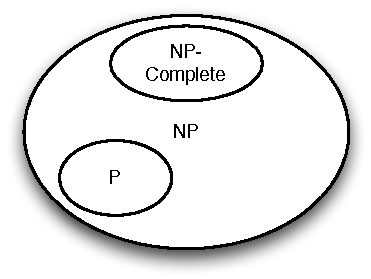
\includegraphics[width=0.5\textwidth]{figures/fig5.pdf}
\caption{Set illustration of the 3 classes of problems. Note that both $P$ and $NPC$ is in $NP$, but they are disjoint i.e. this illustration assumes that $P \neq NP$}
\label{fig5}
\end{figure}

\begin{theorem}
Let $L_1$ and $L_2$ be languages such that $L_1 \leq_p L_2$. Then if $L_2 \in P$ then $L_1 \in P$  
\label{theorem1}
\end{theorem}

\begin{proof}
We know that $L_2$ can be solved in polynomial time. From \ref{eq15} we know that there exist a function $f$ such that $x \in L_1 \Leftrightarrow f(x) \in L_2$. For any $x \in L_1$ we can thus use the result $f(x) in L_2$ and find the answer to the instance $x$. $L_1$ can thus be solved in polynomial time.  
\end{proof}

\begin{theorem}
If any NP-complete problem is solvable in polynomial time, all NP-complete problems are solvable in polynomial time.
\end{theorem}

\begin{proof}
  Suppose that $L \in P$ and also that $L \in NPC$. For any $L' \in NP$ we have $L' \leq_p L$, by property \ref{prop20} of NP-completeness. Since $L \in P$ there must exist a polynomial algorithm. And by \ref{theorem1} this implies that $L' \in P$.
\end{proof}



% subsection definition_of_classes (end)

\subsection{Example $HAM-CYCLE \leq_p TSP$} % (fold)
\label{sub:subsection_name}
In this example we wish to prove that it is very unlikely that a polynomial algorithm exist for the Traveling Salesman Problem (TSP). In fact, we wish to show that solving the TSP is at least as hard as solving the Hamiltonian cycle. We know that the Hamiltonian cycle problem is NP-complete. 

Recall that a Hamilton cycle is a path in a undirected graph where each vertex is visited exactly once.

Thus, if we can show that it is at least as hard to solve the TSP problem as it is to solve the Hamilton cycle program, we have shown that TSP is in the NP-complete class. 

Let the language of the TSP be defined as

\begin{align*}
TSP = \{\langle G, c, k \rangle : & G = (V,E) \text{ is a complete graph}, \\ 
                                  & c:V \times V \rightarrow \Z, \\
                                  & k \in \Z, \\
                                  & \text{$G$ has a TSP tour of at most cost $k$}\}
\end{align*}


We need to show two things. First we need to show that the TSP decision problem is in the NP class. This can be shown by showing that TSP has a verification algorithm, that can verify an instance in polynomial time. 

Let the verification algorithm check the sequence of vertices and sums the total cost and verifies this as being $\leq k$. Such a verification algorithm definitely exist, and can be run in polynomial time.

The next thing we need to show is $HAM-CYCLE \leq_p TSP$. 

Let $G=(V,E)$ be an instance of $HAM-CYCLE$. We can construct an instance of TSP as follows. Form the complete graph\footnote{A complete graph has a path from every vertex to all other vertices.} $G' = (V,E')$. Let the vertices in $V$ be the cities in the TSP. Let the cost function, $c(i,j)$ be defined by

\begin{equation} 
c(i,j) = 
\left\{
\begin{array}{rl} 
  0 & \text{if } (i,j) \in E \\
  1 & \text{if } (i,j) \notin E 
\end{array} 
\right. 
\end{equation} 
So if a edge resides in the Hamilton graph $G$, then it has cost $0$ in $G'$ otherwise $1$. An instance of TSP is thus a cycle in $G'$ with cost at most $0$.

It is clear that we can construct $G'$ in polynomial time. We now show that $G$ contains a Hamilton cycle if and only if graph $G'$ has a tour of cost $0$. Suppose $G$ has a Hamilton cycle $h$. Each edge in $h$ resides in $G$ thus having cost $0$ in $G'$. Conversely, suppose $G'$ has a tour $h'$ of cost $0$, since the cost of the edges in $G'$ is $0$ and $1$, $h'$ can only occur if it traverses the edges of $G'$ with $0$ cost, thus $h'$ contains only edges from $E$.  

We have now proven that finding TSP tour is at least as hard as finding a Hamilton cycle, which concludes that TSP is NP-complete (Since the Hamilton-Cycle problem is NP-complete)
% subsection subsection_name (end)

% section np_completeness (end)
\clearpage \newpage
\section{Branch and Bound and Meta-heuristics} % (fold)
\label{sec:branch_and_bound_and_metaheuristics}

\subsection{Disposition Branch and Bound and Meta-heuristics} % (fold)
\label{sub:disposition_branch_and_bound_and_meta_heuristics}
\begin{itemize}
  \item Motivation: solve hard discrete problems, large search space
  \item Draw solution tree, explain the search space, prune, incumbent etc.
  \item Illustrate branching by independent set, and calculate running time
  \begin{itemize}
    \item Recurrence: \begin{equation}
      T(n) \leq 1 + T(n-d(v)-1) + \sum_{i=1}^{d(v)} T(n-d(v_i)-1)
    \end{equation}
    \item Algorithm alway choses vertex with minimum degree so  
    \begin{equation}
      T(n-d(v)-1) \geq T(n-d(v_i)-1)      
    \end{equation}
    \item Merge the sums
    \item let $s = d(v)+1$
    \item Expand 
    \begin{equation}
      t(n) \leq 1 + sT(n-s) \leq 1 + s + s^2+s^3+\ldots+s^{n/s} 
    \end{equation} to $\O(S^{n/s})$ <- harmonic series.
  \end{itemize}  
  \item Bounding by TSP and 1-tree
  \begin{itemize}
    \item Lower bound on TSP
    \item Pick node
    \item Remove all incident edges
    \item make minimum spanning tree
    \item Add smallest two edges to minimum spanning tree, cost is lower bound
  \end{itemize}
  \item TSP Root node fully connected graph
  \item Branch on nodes with degree 3 or more
  \item lower bound is increased every time we branch.
  \item Meta heuristic algorithms
  \begin{itemize}
    \item Hill Climbing <- Steepest descent
    \item Tabu search <- Memory
    \item Simulated annealing <- Accepts non improving solutions with a certain probability
  \end{itemize}
\end{itemize}
% subsection disposition_branch_and_bound_and_meta_heuristics (end)
\newpage

\subsection{Motivation} % (fold)
\label{sub:motivation}
NP-hard problems can be solved to closed form by using an exact algorithm like branch and bound. They can be solved heuristically by using meta algorithms.

The search space for NP-hard problems are extremely large, and solving problems exact means, to some extent, that we need to traverse the whole search space. Solving heuristically means to traverse part of the search space, thereby gaining a speedup. 

By using branch and bound we are trying not to visit the whole solution space, but instead only visit the solution space where we know an optimal solution could reside. Suppose we have a problem, with tree binary variables $x_1, x_2, x_3$. Figure \ref{fig21} shows a total enumeration tree for this problem. There are in total $2^3 = 8$ solutions, and in general we can describe the number of solutions to such a problem as $2^n$.

This is an example of a problem where we do not want to explore the whole search tree before we find a solution. Imagine we could prune some branches of the tree, thereby making the search tree smaller. This is exactly what Branch \& Bound does.

The nodes of a Branch \& Bound tree corresponds to partial solutions, i.e solutions where some part of the variables are defined and some part is not. The leafs corresponds to solutions where all the variables are defined.

A bounding function takes partial solution, and from this calculates a bound on the complete solution containing this partial solution.

The incumbent is the best known feasible solution found so far. One wishes to find an incumbent as fast as possible, as this means that, hopefully, some parts of the tree will have a bound worse than the incumbent, thereby giving us the possibility to discard these parts.

By the help of the bounding function, we can calculate the a bound of a node containing a partial solution. If this bound is worse than the incumbent, then we can discard this part of the tree, thereby remove parts of the search space.

\begin{figure}[ht]
\centering
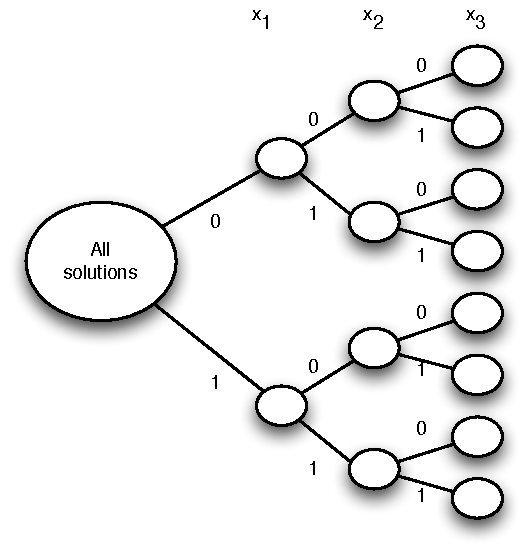
\includegraphics[width=0.5\textwidth]{figures/fig21.pdf}
\caption{Total enumeration of solutions, for a problem with tree binary variables $x_1, x_2, x_3$. The leafs of the tree corresponds to solutions, whereas the node is partial solutions}
\label{fig21}
\end{figure}
% subsection motivation (end)

\subsection{Branching} % (fold)
\label{sub:branching}
The branch part of the Branch and Bound algorithm divides the problem into subproblems

In order to illustrate branching we can use the problem of finding the independent set in a graph. 

Given a graph $G = (V,E)$ the independent set is the set of vertices $I \subset S$, such that for every vertex in $I$ none of it's neighbors in $V$ are in $I$. I.e. each edge in $E$ has at most one endpoint in $I$. The maximal independent set, is a set independent set where $|I|$ is maximized.

A trivial algorithm to find such a set, is to construct all possible solutions by permutation, and check if it is a independent set. The running time can be calculated from the following observation. Each vertex in the graph can either be included in the set or not included in the set. For each vertex we thus have 2 possibilities. Given $n$ vertices this yields a running time of $\O(2^n)$!

Another approach is to use a branching algorithm. The branching algorithm works as follows. Given a graph $G = (V,E)$ pick a vertex, $v$ with minimum degree\footnote{A degree of a vertex $v$ is the number of adjacent edges to $v$}. Let the set of neighbors to $v$ be defined as $N[v]$. For each vertex $j \in N[V]$ do a branch on the set $G \setminus N[j]$.

Figure \ref{fig20} illustrates an example run of the independent set algorithm.

\begin{figure}[ht]
\centering
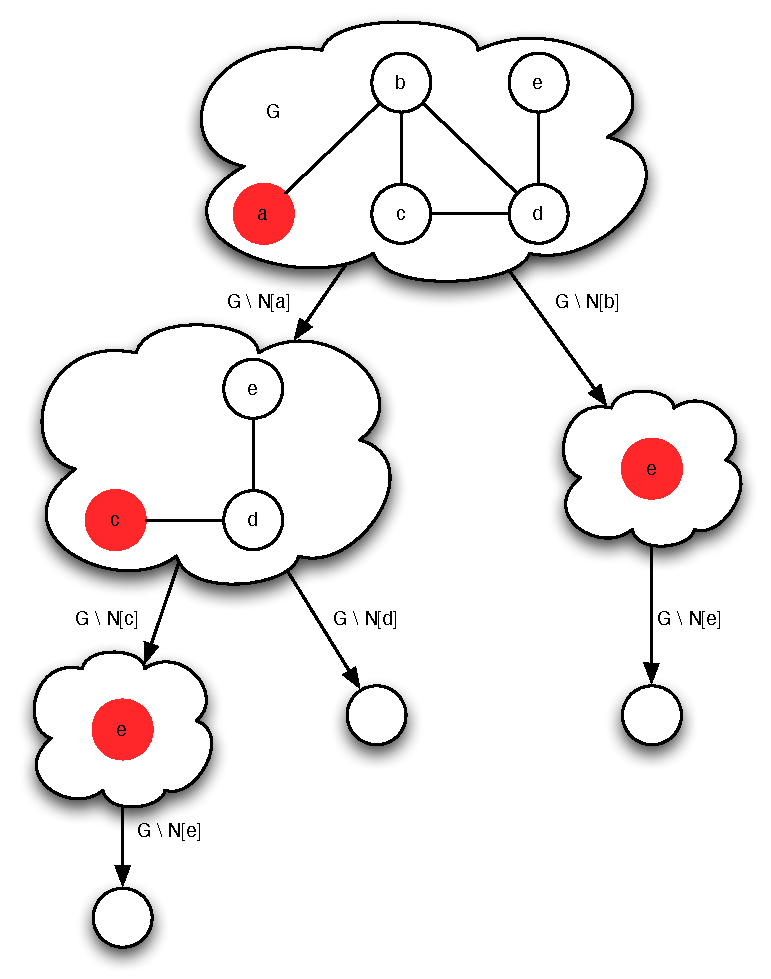
\includegraphics[width=0.50\textwidth]{figures/fig20.pdf}
\caption{Example run of the independent set algorithm}
\label{fig20}
\end{figure}


The running time of this procedure can be calculated as the number of nodes in the search tree $T$. The algorithm picks the vertex with the minimum degree and branches on itself and it's neighbors. We thus have

\begin{equation}
  T(n) \leq 1 + T(n-d(v)-1) + \sum_{i=1}^{d(v)} T(n-d(v_i)-1)
\end{equation}
where $d(v_i)$ is the degree of the $i'th$ neighboring vertex. 

Since the algorithm always chooses the vertex with minimum degree we have $T(n-d(v)-1) \geq T(n-d(v_i)-1)$. so
\begin{align}
T(n) &\leq 1 + T(n-d(v)-1) + \sum_{i=1}^{d(v)} T(n-d(v_i)-1) \\
     &\leq 1 + T(n-d(v)-1) + \sum_{i=1}^{d(v)} T(n-d(v)-1)   \\
     &= 1 + \sum_{i=1}^{d(v)+1} T(n-d(v)-1)                  \\
     &= 1 + (d(v)+1)T(n-d(v)-1)          
\end{align}
now let $s = d(v)+1$ then we have
\begin{equation}
  t(n) \leq 1 + sT(n-s)          
\end{equation}
expanding this recurrence yields
\begin{equation}
  t(n) \leq 1 + sT(n-s) \leq 1 + s + s^2+s^3+\ldots+s^{n/s}  \label{brancheq1}       
\end{equation}
this follows from the observation, that we subtract $s$ from $n$ at each recursive step, so the maximal number of recursive steps is $n/s$. \ref{brancheq1} is a harmonic series and can be written as $\O(s^{n/s})$.
% subsection branching (end)


\subsection{Bounding} % (fold)
\label{sub:bounding}
The bounding part of the Branch and Bound algorithm gives a bound of the partial solution found so far. In order to illustrate the bounding part, I have chosen to use the TSP problem. 

Given a TSP problem let the root node be the fully connected graph. We can calculate a lower bound of the TSP tour by the following procedure. Choose a special node $\#1$ and remove all it's incident edges. Calculate the minimum spanning tree, $t_{rest}$ of the rest of the graph. Add the two shortest edges $e_1,e_2$ incident to $\#1$ $t_{rest}$ producing $t_{one}$. $t_{one}$  is now a 1-tree. 

\begin{definition}
The total cost of $t_{one}$ is less than the total cost of the optimal tour.  
\end{definition}

\begin{proof}
  Note that a Hamilton cycle in $G$ consist of two edges $e'_1$, $e'_2$ and a tree $t'_{rest}$ in the rest of $G$. So the set of Hamilton cycles is a subset of the set of 1-trees. Since $e_1$ and $e_2$ are the shortest edges incident to $\#1$, and $t_{rest}$ is the minimum spanning tree in the rest of $G$, the cost of $t_{one}$ is less than or equal to the cost of any Hamilton cycle, especially a TSP tour.
\end{proof}

The root node of the Branch and Bound search tree of the TSP is the fully connected graph. Every time we branch on a node $j$, we remove edges from $G$ so they are not present in the descendants of $j$. We branch on all the nodes which has degree $\geq 3$.

How to get an initial Incumbent brings us to meta-heuristics

% subsection bounding (end)


\subsection{Meta-Heuristics} % (fold)
\label{sub:heuristics}

Meta-heuristic algorithms is algorithms that try to find a optimal solution, by improving a previous solution. Most heuristic methods starts with an initial solution, and permutes it slightly thereby giving a new, possible better, solution. 

The difference between heuristic algorithms and approximation algorithms is that the approximation algorithms gives a guarantee of the result, whereas the heuristic algorithms does not give this guarantee.  

All the algorithms presented below, needs an initial solution. It really depends on the problem how this initial solution is found. For the TSP problem the nearest neighbor algorithm could be used or alternatively calculating the convex hull and adding points to the edges of the hull.

Furthermore, the description of the neighborhood is very problem specific.

\subsubsection{Hill climbing} % (fold)
\label{ssub:hill_climbing}
Hill climbing is a simple heuristic algorithm that only makes strictly improving moves. Given a initial solution $s$, a sample is chosen from the neighborhood, $t \in N(s)$. If the sample yields a better solution, then the initial solution is exchanged with the sample i.e $s=t$. This procedure is repeated until local optima is reached, i.e. 

\begin{equation}
  f(t) \leq f(s) \qquad \forall t \in N(S)
\end{equation}

The problem with Hill climbing is that local optima doesn't guarantee to bee close to the global optima, actually it could be far away from the global optimum.

% subsubsection hill_climbing (end)

\subsubsection{Simulated annealing} % (fold)
\label{ssub:simulated_annuealing}
Simulated annealing is a heuristic algorithm that always performs improving moves, but also accept non improving moves. The algorithm has a tweaking parameter $T$ that is gradually decreased as the algorithm runs. Given a initial solution, $s$ and a initial tweaking parameter $T$ the algorithm chooses a sample, $t$ from the neighborhood. If the sample yields a better solution, the initial best solution is discarded and replaced by the sample. If the sample does not yield a better solution, the sample is accepted with probability
\begin{equation}
  e^{\frac{s-t}{T}}
\end{equation}
% subsubsection simulated_annuealing (end)


\subsubsection{Tabu search} % (fold)
\label{ssub:tabu_search}
Tabu search is a heuristic algorithm that has memory. It memorizes the places it has already visited, and forbids the algorithm to visit these places again. This has the effect that no cycling can occur, and no solution is explored twice. 

Otherwise the algorithm works as Hill climbing, where the best solution is replaced if the candidate solution is better.
% subsubsection tabu_search (end)
% subsection heuristics (end)


% Branch and Bound and Metaheuristics are  distributed notes ([Clausen] sections 1 and 2], [Luke] sections 0,1 and 2, [Fomin and Kratsch] chapter 1 and chapter 2).                                                                                                                                                          
% section branch_and_bound_and_metaheuristics (end)
\clearpage \newpage
\section{Approximation Algorithms} % (fold)
\label{sec:approximation_algorithms}

\subsection{Disposition Approximation Algorithms} % (fold)
\label{sub:disposition_approximation_algorithms}
\begin{itemize}
  \item Difference between Heuristic algorithms
  \item Performance ratio $max(\frac{C}{C^*}, \frac{C^*}{C})$
  \item 2-approximation algorithm for the vertex cover problem
  \begin{itemize}
    \item Put lover bound of optimal solution, each edge must have a single node in the vertex cover
    \item Let $A$ be the set of edges picked in the approximation algorithm
    \item Then $C* \geq |A| \Leftrightarrow 2C* \geq 2|A|$, i.e. each edge must have one node in the optimal set cover
    \item The approximation algorithm adds two edges every time it picks one from $A$, thus $C = 2|A|$
    \item Substituting yields $2C* \geq 2|A| = 2C* \geq C$
  \end{itemize}
  \item 2-approximation algorithm for the TSP problem
  \begin{itemize}
    \item Let H* be a TSP tour, now remove one edge, yielding a minimum spanning tree $T$. Thus the cost of the spanning tree is a lower bound 
    \begin{equation}
    c(T) \leq c(H*) \Leftrightarrow = 2c(T) \leq 2c(H*)
    \end{equation}
    \item Imagine instead of a pre-order tree walk, we did a full walk, $H'$, thus the walk would cost $c(H') = 2C(T)$
    \item By removing vertices from $H'$ we are only making the tour shorter (Triangle inequality)
    \item Combining yields $2c(T) \leq 2c(H*) \Leftrightarrow c(H') \leq 2c(H*) $
  \end{itemize}
  \item Set cover problem $\rho(n) = ln(n)$
  After the first iteration we would have at least 
  \begin{equation}
  r_1 = r_0-r_0/opt=r_0(1-1/opt)  
  \end{equation}
  points left to cover.  
  At each iteration we pick a set, so $k$ yields the number of sets we have picked. How many iterations do we have to do before there are no more sets to pick? 
  \begin{align}
  r_0(1-1/opt)^k < 1 \\
  \end{align}
  Which by some tricks can be reduces to $k < opt\log(r_0)$. Thus all elements are covered after selecting greedily at most $OPT \O(\log(r_0))$ sets.
\end{itemize}
% subsection disposition_approximation_algorithms (end)
\newpage

\subsection{Performance ratio} % (fold)
\label{sub:performance_ratio}
The performance ratio, $\rho(n)$ is defined as
\begin{equation}
  max(\frac{C}{C^*}, \frac{C^*}{C}) \label{eqapprox0} \leq \rho(n)
\end{equation}
where $C^*$ is the cost of the optimal overall solution, $C$ is the cost of the solution found by the approximation algorithm and $n$ is the number of elements. The definition of the ratio applies both to maximization and minimization problems. 

In a maximization scenario typically $0 < C \leq C^*$, and $C^*/C$ gives the factor by which the cost of $C^*$ is greater than the cost of $C$. In a minimization scenario $0 < C^* \leq C$ and $C/C^*$ tells by which factor $C$ is greater than $C^*$.

If an algorithm archives an ratio of $\rho(n)$ then we call the algorithm a $\rho(n)$-approximation algorithm.

As can be seen from the definition, a ratio is equal to $1$ when the cost of the optimal and the approximation is equal. This scenario corresponds to the case where the approximation equals the optimal solution.

Example: Imagine an approximation algorithm that has a worst case of twice the optimal solution disregarding the input size $n$. Then the approximation factor would be $\rho(n)=2$.
% subsection performance_ratio (end)


\subsection{The vertex cover problem} % (fold)
\label{sub:the_vertex_cover_problem}

A vertex cover of an undirected graph $G=(V,E)$ is the problem of finding the subset of vertices $V' \subset V$ such that $\forall (u,v) \in E: u \in V' \vee v \in V'$, i.e. each edge is connected to a vertex in $V'$. The size of the vertex cover is the number of vertices in $V'$. The vertex cover problem is finding a vertex cover of minimum size. The vertex cover problem is NP-complete. 

The approximation algorithm for vertex cover is a polynomial algorithm and works as follows: Let the input to the algorithm be a undirected graph $G = (V,E)$. Let $E' = E$ be the edges of the graph. While there are edges in $E'$ pick a edge $(u,v)$ from $E'$. Add the vertices $u$ and $v$ to the final vertex cover set $C$. Remove from $E'$ every edge incident to either $u$ or $v$.

An example run can be seen in figure \ref{fig12}

\begin{figure}[ht]
\centering
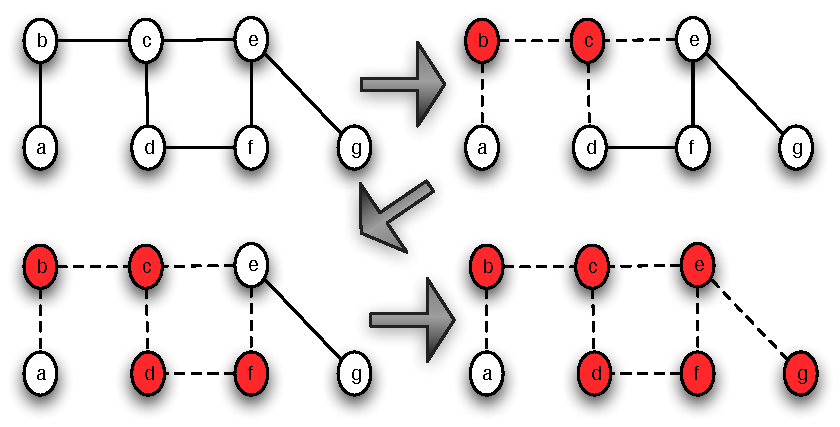
\includegraphics[width=0.75\textwidth]{figures/fig12.pdf}
\caption{Example run of the approximated vertex cover algorithm. The value is 6.}
\label{fig12}
\end{figure}

Figure \ref{fig13} shows the optimal solution
\begin{figure}[ht]
\centering
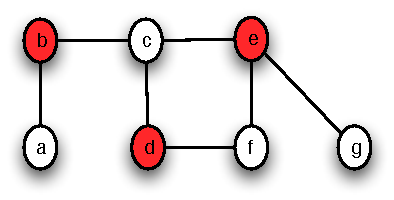
\includegraphics[width=0.5\textwidth]{figures/fig13.pdf}
\caption{Optimal solution to the vertex cover problem. The value is 3.}
\label{fig13}
\end{figure}

The approximated vertex cover algorithm is a polynomial time 2-approximation (It is a polynomial time algorithm and the approximation ratio is 2.).

\begin{proof}
Let $A$ be the set of edges that is picked in the approximation algorithm. Let $C*$ be the optimal vertex cover. Let $C$ be the vertex cover generated by the approximation algorithm. 

We can put a lower bound on $C^*$ as follows. The number of elements in $C^*$ must be at least $|A|$. This follows from the following observation: Each edge in $A$ must have one of it's vertices in $C^*$, otherwise we would have a edge not in $C^*$, and therefore an edge not part of the vertex cover which contradicts our assumption that $C^*$ was a optimal vertex cover. Thus $|C^*| \geq |A|$. For convenience, we will rewrite this lower bound as 
\begin{equation}
|C^*| \geq |A| \Leftrightarrow 2|C^*| \geq 2|A|  \label{vertexcovereq1}
\end{equation}

Every time the approximation algorithm picks an edge from $A$, it adds two vertices to $C$. Therefore 
\begin{equation}
|C| = |2A| \label{vertexcovereq2}   
\end{equation}

Substituting \ref{vertexcovereq2} in \ref{vertexcovereq1} yields
\begin{equation}
2|C^*| \geq |C|
\end{equation}
thereby giving us a upper-bound on the number of elements in the vertex cover found by the approximation algorithm.
\end{proof}

% subsection the_vertex_cover_problem (end)


\subsection{The TSP problem} % (fold)
\label{sub:the_tsp_problem}
In the following we assume that the triangle inequality\footnote{Intuitively explanation: The shortest distance between 2 points is always a straight line} holds. If the triangle inequality do not hold, then it is possible to show that no polynomial approximation algorithm exists!

The TSP problem can be solved by a 2-approximation polynomial algorithm. The algorithm works as follows. It takes a bunch of points, and makes a complete graph. It then runs Prim's algorithm to find the minimum spanning tree\footnote{Tree containing all the vertices where the length of the edges is minimized. Running time depends on implementation but can be $\O(E\log(V))$ when using a binary heap}

After finding the minimum spanning tree we have a list of vertices contained in a binary heap. We then create a list, $H$ from the pre-order tree walk of this binary heap. The pre-order tree walk can be thought of as we are walking along side the minimum spanning tree, always having the vertices to the left of the current direction. Each time we meet a vertex we haven't seen before, we store it in $H$. Eventually we will return to the starting node. 

$H$ is the approximated solution to the TSP problem. An example run can be seen on figure

\begin{figure}[ht]
\centering
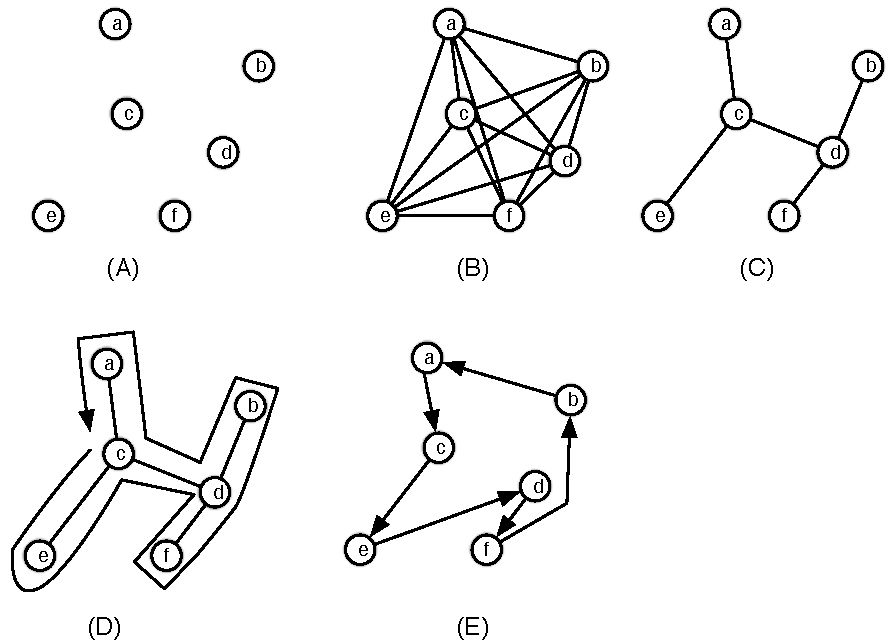
\includegraphics[width=0.75\textwidth]{figures/fig14.pdf}
\caption{Example run of the TSP approximation algorithm. (A) initial point cloud. (B) Fully connected graph. (C) Minimum spanning tree. (D) pre-order tree walk. (E) Approximated TSP tour}
\label{fig14}
\end{figure}


The approximated TSP tour is a polynomial time 2-approximation algorithm. I.e. the approximation algorithm is maximum twice as `bad' as the optimal solution.

\begin{proof}
The proof is similar to the proof given for the vertex cover problem. We start by showing a lower bound of the optimal tour. Let $H^*$ be a TSP optimal tour. Now remove one edge from $H^*$ we now have a minimum spanning tree. Therefore the total cost of the spanning tree, $T$, computed in the algorithm above is a lower bound of the optimal TSP tour i.e.

\begin{equation}
  c(T) \leq c(H^*) \Leftrightarrow 2c(T) \leq c(H^*) \label{tspeq1}
\end{equation}

Imagine instead of a pre-order tree walk we did a full walk, adding a node to $H$ every time we encountered it disregarding if we have seen the node before. We would then end up with a list of vertices $H'$ where the vertices where allowed to be present multiple times. The full walk traverses every edge in $T$ exactly twice, we have

\begin{equation}
  c(H') = 2 c(T) \label{tspeq2}
\end{equation}
i.e. the cost of the full walk is twice the cost of the minimum spanning tree. 

We now put the triangle inequality in to play. The triangle inequality states that the shortest path between two nodes is the direct path. I.e. if we remove nodes from $H'$, the cost would decrease. 

Now create a new list $H$ from $H'$ where the elements in $H$ is the unique elements in $H'$ in the order they are present in $H'$. If we compare the cost of $H$ and $H'$ it is clear that 
\begin{equation}
  c(H) \leq c(H') \label{tspeq3}
\end{equation}

Combining \ref{tspeq1}, \ref{tspeq2} and \ref{tspeq3} we arrive at
\begin{equation}
  c(H) \leq c(H') \leq 2c(H^*)  
\end{equation}
which concludes the proof.

\end{proof}

There exist no approximated solution if the cost function doesn't satisfy the triangle inequality. This follows from the following argumentation: If there where such an approximated polynomial solution with $\rho>1$ then we could use this approximated solution to solve the Hamilton cycle problem, and since the Hamilton cycle problem is NP-complete this is highly unlikely as we assume the $P \neq NP$. The proof uses reduction to turn the Hamilton cycle problem into the TSP problem, and utilizing that disregarding the size of $\rho$ the algorithm most return a Hamilton cycle.
% subsection the_tsp_problem (end)

\subsection{Set covering problem} % (fold)
\label{sub:set_covering_problem}
Given a set of elements $X$ and a set of subsets $F$ where each element in $F$ is a subset of $X$ we wish to find the minimum number of subsets in $F$ where the union of these is equal to $X$. Formally we seek a set of subsets, $F^*$, where
\begin{equation}
\bigcup_{f \in F^*} f= X
\end{equation}
and where $|F^*|$ is minimized.

The problem of finding such a set is NP-complete.

Figure \ref{fig15} shows an instance of the set cover problem.

\begin{figure}[ht]
\centering
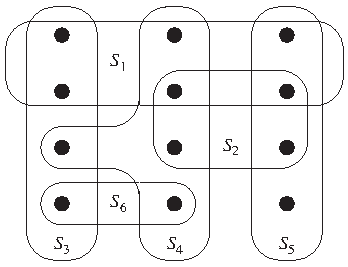
\includegraphics[width=0.75\textwidth]{figures/fig15.pdf}
\caption{Instance of the set cover problem, where $X$ consist of the 12 black marks, and $F = \{s_1, s_2, s_3, s_4, s_5, s_6\}$. The greedy algorithm, would start by selecting $s_1$, then $s_4$ and $s_5$ and finally either $s_3$ or $s_6$ would be picked in that order. The optimal solution is $s_3, s_5, s_6$}
\label{fig15}
\end{figure}

The greedy-set-cover algorithm is an approximation algorithm. It works as follows 
\begin{alltt}
Greedy-set-cover(X,F)\{
  U = X
  F = \(\emptyset\)
  while(U != \( \emptyset \))\{
    Pick the set \(S \in F\) such that \( | S \cap U | \) is maximized
    F = F \(\cup\) \{S\}
    U = U - S
  \}
  return F  
\}
\end{alltt}

Let $OPT$ denote the number of sets in the optimal solution. Let $r_i$ denote the number of uncovered elements after the $i'th$ iteration. Initially $r_0 = n$ where $n$ is the number of elements. The algorithm picks at least a set covering $r/OPT$ elements at every iteration. 

After the first iteration we would have at least 
\begin{equation}
r_1 = r_0-r_0/opt=r_0(1-1/opt)  
\end{equation}
points left to cover. 

After the second iteration we would have at least $r_1(1-1/opt)$ points to cover. Expanding these expressions yields that after the $k'th$ iteration we would have at least 
\begin{equation}
  r_0(1-1/opt)^k  
\end{equation}
points to cover.

At each iteration we pick a set, so $k$ yields the number of sets we have picked. The question now is, how many iterations do we have to do before there are no more sets to pick? This question can be answered with the following inequality

\begin{align}
r_0(1-1/opt)^k < 1 \\
\end{align}
Which by some tricks can be reduces to $k/opt > log(r_0)$. Thus all elements are covered after selecting greedily at most $OPT \O(\log(r_0))$ sets.
% subsection set_covering_problem (end)

\subsection{Linear program to vertex cover} % (fold)
\label{sub:linear_program_to_set_cover}
Approximate vertex cover an alternative way. Linear programming can be used in approx. algorithms. We want to solve vertex cover in a "weighted" version, called weighted vertex cover. Instead of wanting to archive the minimum number of nodes, we want to archive the minimum weight of the nodes.

Let every node $v_n$ have a weight $w(v_n)$. Goal: To minimize the total weight $\sum_{\forall v \in V} w(v)$ in the vertex cover. 

We need to express the problem in terms of integer programming. Thus
\begin{equation}
\sum_{\forall v \in V} w(v) x(v)  
\end{equation}
where $x(v)=1$ if vertex is in cover otherwise $0$. Subject to
\begin{equation}
  x(u)+x(v) \geq 1 \qquad \forall (u,v) \in E
\end{equation}
(At least one of two adjacent vertices has to be in vertex cover.) and
\begin{equation}
    x(v)  \in \{0,1\} \qquad \forall v \in V 
\end{equation}

We need to transform the integer programming problem into a linear program by relaxing the last constraint, i.e. $0 \leq x(v) \leq 1 \qquad \forall v \in V$. This linear program can be solved optimal in polynomial time. 

The linear program can be related to the integer program as follows: The linear program gives us at least the value of the integer programming problem. The linear program is thus a lower bound of the integer program.
% subsection linear_program_to_set_cover (end)

\subsection{Subset-sum problem} % (fold)
\label{sub:subset_sum_problem}
There are two problems known as the subset sum problem: An optimization and a decision problem. The decision problem is as follows:

\begin{definition}
Given a set of integers and an integer $s$, does any non-empty subset sum to $s$?  
\end{definition}
the optimization is as follows
\begin{definition}
Given a set of integers and an integer $s$, find a subset of of the integer set so that the sum of the subset is as close to $s$ as possible.
\end{definition}
In both cases the problem is NP-complete.


An exact solution to the subset sum problem is the following algorithm. 

\begin{alltt}
Exact-subset-sum(S,t)\{
  n = |S|
  \(l_0\) = \{0\}
  for(i=1 to n)\{
    \(l_i\) = MergeList(\(l_{i-1},l_{i-1}+x_i\))  <- add \(x_i\) to every element in \(l_{i-1}\)
    remove from \(l_i\) all elements greater than t.
  \}
  return max(\(l_n\))
\}  
\end{alltt}
where \texttt{MergeList(x,y)} as a procedure that merges to list, sorting them in decreasing order an removing duplicates. An example with $S = \{1, 4, 5\}$ yields

\begin{alltt}
\(l_0\) = \{0\}
\(l_1\) = \{0,1\}
\(l_2\) = \{0,1,4,5\}
\(l_3\) = \{0,1,4,5,6,9,10\}
\end{alltt}

The list $l_i$ can grow exponential large, up to $2^i$.

The following is a approximation algorithm that returns a value within $1+\epsilon$ factor of the optimal solution. The idea is to trim the list after each iteration, such that if some elements in the list are within a certain threshold of each other, only the smallest element is retained. 

More precisely, given an element $e_i$ in the list, the next element is removed if $(1+\epsilon)e_i\geq e_{i+1}$ then $e_{i+1}$ is removed. This trimming can be done in $\O(m)$ where $m$ is the length of the lust given to the trim function.

\begin{alltt}
Approx-subset-sum(S,t)\{
  n = |S|
  \(l_0\) = \{0\}
  for(i=1 to n)\{
    \(l_i\) = MergeList(\(l_{i-1},l_{i-1}+x_i\))  <- add \(x_i\) to every element in \(l_{i-1}\)
    \(l_i\) = Trim(\(l_{i},\epsilon/2n\))            <- remove similar elements
    remove from \(l_i\) all elements greater than t.
  \}
  return max(\(l_n\))
\}  
\end{alltt}

The trimming of the list is done so it won't grow exponentially. On one hand it keeps only a polynomial number of elements in the list, but at the same time the allowed error is so small, that although it may increase at each step, it still does not add to something which is so big that it violates the required approximation bound.


% subsection subset_sum_problem (end)


% section approximation_algorithms (end)
\clearpage \newpage
\section{Randomized Algorithms} % (fold)

\subsection{Disposition Randomized Algorithms} % (fold)
\label{sub:disposition_randomized_algorithms}
\begin{itemize}
  \item Motivation, eliminate the worst enemy problem etc.
  \item 2 ways to randomize
  \begin{itemize}
    \item Permute by shorting, $\O(n\log(n))$
    \item Permute in place, $\O(n)$
  \end{itemize}
  \item Quicksort - Avoid pivoting on largest element
  \item Binary search tree - avoid skew tree
  \item Selection algorithm - Avoid pivoting on largest element
\end{itemize}
% subsection disposition_randomized_algorithms (end)

\newpage

\label{sec:randomized_algoritms}
Randomized algorithms, are algorithms that seeks to eliminate the possibility that `your worst' enemy gives you a input such that the algorithm runs slowly.

\subsection{Hiring problem} % (fold)
\label{sub:hiring_problem}
Say we want to hire a person. We have a external company that gives us the names of the candidates we wish to interview. Each candidate is assigned an integer value describing how good the candidates qualifications are. If the candidate is better qualified i.e. here value is greater than the candidate we presently have, she is hired.

Each time we hire a candidate it cost us money. Interviewing has zero cost.

Now we want to minimize the total cost, when interviewing $n$ candidates. We need to interview all candidates, but every time a new candidate with better qualifications comes around, we need to hire her, and fire the previous. If we have no control over the ordering the candidates arrive in, we risk the situation where the candidates arrive in sorted increasing order by their value. This would mean that we would have to hire all $n$ candidates! The worst case is thus a total cost of $\O(cn)$ where $c$ is the cost of hiring a single candidate.

A randomized approach to this problem would be to receive the full list of candidates from the external company, randomize the list, and call in the candidates in the randomized order. This would eliminate the possibility that the candidates where interviewed in a predetermined manner.

Because the candidates arrive in randomized order, and each candidate is equally likely to be the best, we have that the probability that the $i'th$ candidate is hired can be expressed as $1/i$.

From the harmonic series we have the cost as $1/1+1/2+1/3+\ldots+1/n \approx \ln(n)$ which is also the \emph{expected} cost of the algorithm. 

In order to arrive at this result we used the \emph{linearity of expectations}. Linearity of expectations means that the expected value of a sum equals the expected value of each $i'th$ terms of the sum. Dice example.Throwing a dice yields a number in the interval $1-6$. The expected number is $3,5$. Throw the dice 10 times then the expected sum will be 35. This holds only for summation not products. For products it only holds for unrelated events (iid).


% subsection hiring_problem (end)

\subsection{Randomization} % (fold)
\label{sub:randomization}
Many algorithms take as input an array of data. This data can be randomized in several ways. Two methods are described here. In both cases it is worth noticing that the probability of the random generator is uniform! 

\subsubsection{Permute by sorting} % (fold)
\label{ssub:permute_by_sorting}
Permute by sorting works in the following way. Generate a new array, $P$, with length $n$ where $n$ is the length of the input array $A$. Each entry in $P$ has a random value in the range $[1,n^3]$. Now sort $A$ by the keys of $P$. The complexity of this algorithm is as follows. Generating $P$ takes $\O(n)$. Sorting can be done in $\O(n\log(n))$. The total complexity is thus $\O(n+n\log(n)) = \O(n\log(n))$.

An example of the algorithm is as follows. Given $A = \langle 1,2,3,4\rangle$, we compute $P = \langle 36, 3, 62, 19\rangle$. By sorting $A$ with the keys in $P$ we arrive at $A = \langle 2, 4, 1, 3 \rangle$.
% subsubsection permute_by_sorting (end)

\subsubsection{Randomize in place} % (fold)
\label{ssub:randomize_in_place}
Randomize in place works as follows. Given an array $A$, we swap the $i'th$ element of $A$ with a element picked randomly from the interval $[i,n]$ where $n$ is the number of elements in $A$. This randomization algorithm runs in $\O(n)$.
% subsubsection randomize_in_place (end)

% subsection randomization (end)


\subsection{Quicksort} % (fold)
\label{sub:quicksort}
Quicksort has a worst case running time of $\O(n^2)$. This running time occurs, when the pivot is chosen as the largest element at every iteration. In order to accommodate this problem we can randomize the way we choose the pivot.

The changes to quicksort are small. Instead of always choosing the element in the last position of the array we are currently working on, then choose the pivot at random. We thus swap the last element with a random element from the array and choses this. The only change to the quicksort algorithm is thus the swap procedure. The expected running time is now $\O(n\log(n))$.
% subsection quicksort (end)


\subsection{Binary search tree} % (fold)
\label{sub:binary_search_tree}
A binary search tree is a tree where each node has either none, one or two children. A child positioned to the left of a node has a value less than the node, and a child positioned to the right of a node has a value greater than the node.

The height of the binary search has direct impact of the time it takes to search, insert and delete nodes. Therefore it is desirable that the height is as small as possible, i.e. the binary tree must be balanced.

A binary search tree can be built from an array of values. The first element of the array becomes the root of the tree. The second element becomes a child of the root, and is positioned to the left if it is lesser than the root node, otherwise it is positioned to the right. This procedure poses a problem. If your worst enemy gave you a an array sorted in increasing\footnote{or decreasing, the height is still $\O(n)$} order the binary search tree would have height $n$, where $n$ is the number of elements in the array. This is not tractable! 

The reason is that whenever a new node is inserted to the search tree it is positioned to the right, because the element being inserted is greater than all other elements inserted. An illustration can be seen on figure \ref{fig11}

We can accommodate this problem, by either choosing the element to insert randomly from the array, or totally randomize the array before inserting.

\begin{figure}[ht]
\centering
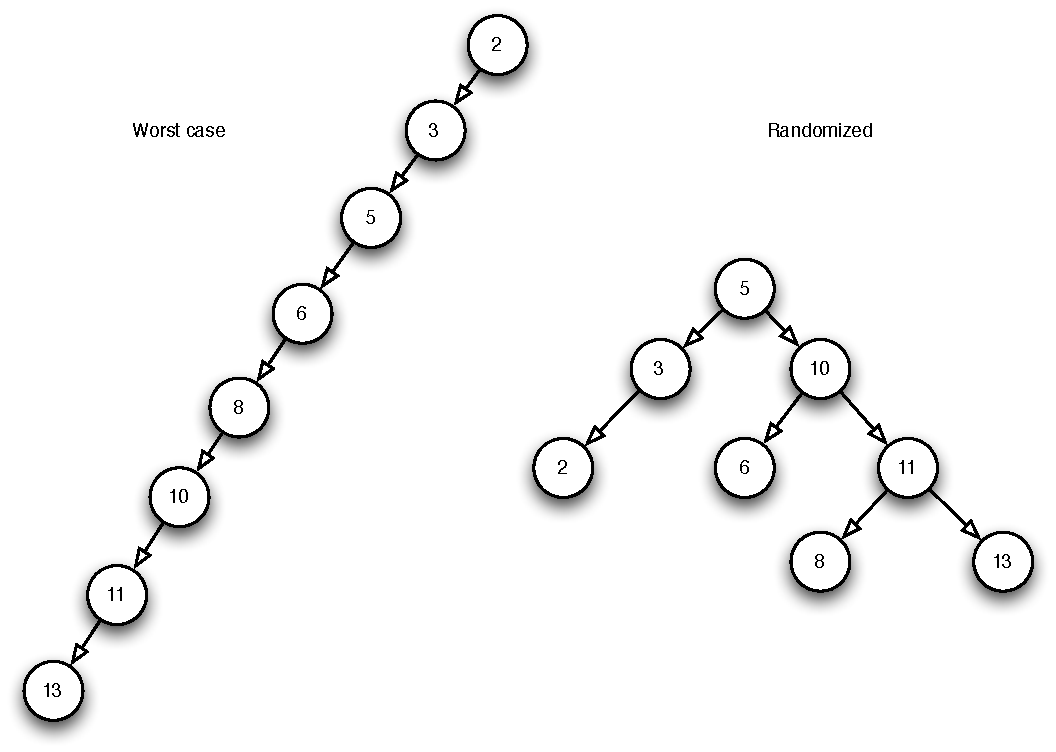
\includegraphics[width=0.75\textwidth]{figures/fig11.pdf}
\caption{Illustration of the difference in height, when using the randomized version, compared to the original version.}
\label{fig11}
\end{figure}

% subsection binary_search_tree (end)

\subsection{Selection algorithm} % (fold)
\label{sub:selection_algorithm}
Randomized select is a randomization algorithm that finds the $i'th$ smallest element in time $\O(n)$. It relies on the randomized partition function also used in quicksort. The problem is again if we keep selecting the largest pivot, we will search through all elements.

The algorithm is recursive and selects a part of the total array where it knows the $i'th$ smallest element is in. Following is the algorithm
\begin{verbatim}
Randomized Select(A, p, r, i){
  if p==r                                       <- Base case
      return A[p]
  q = randomized_partition(A,p,r)               <- Partition A, q is index of pivot
  k = q-p+1                                     <- k is the 
  if k==i
      return A[q]                               <- BINGO
  elseif i<k
      return Randomized Select(A, p, q-1, i)    <- Look in the left part
  else   
      return Randomized Select(A, q+1, r, i-k)  <- Look in the right part
}  
\end{verbatim}
The algorithm starts by checking if the list only consist of $1$ element. Otherwise it does a randomized partition of the list and returning the index of the partitioning in $q$. $k$ can be interpreted as the number of elements between $p$ and $q$. If $k=i$ then we know that the we have found the element, and the element is the same as the pivot element.

If $i<k$ then we know that the $i'th$ element is to the left of the pivot element. We recursively call the function of this part of the list, discarding the current pivot element.

If $i>k$ then we know that the $i'th$ element must lie behind the pivot element, and we thus look at this part of the list. When looking at the right hand side of the list, we need to change $i$ so it becomes $i = i-k$.

Figure \ref{fig10} shows an example run of the algorithm. The expected running time of the algorithm is $\O(n)$.

\begin{figure}[ht]
\centering
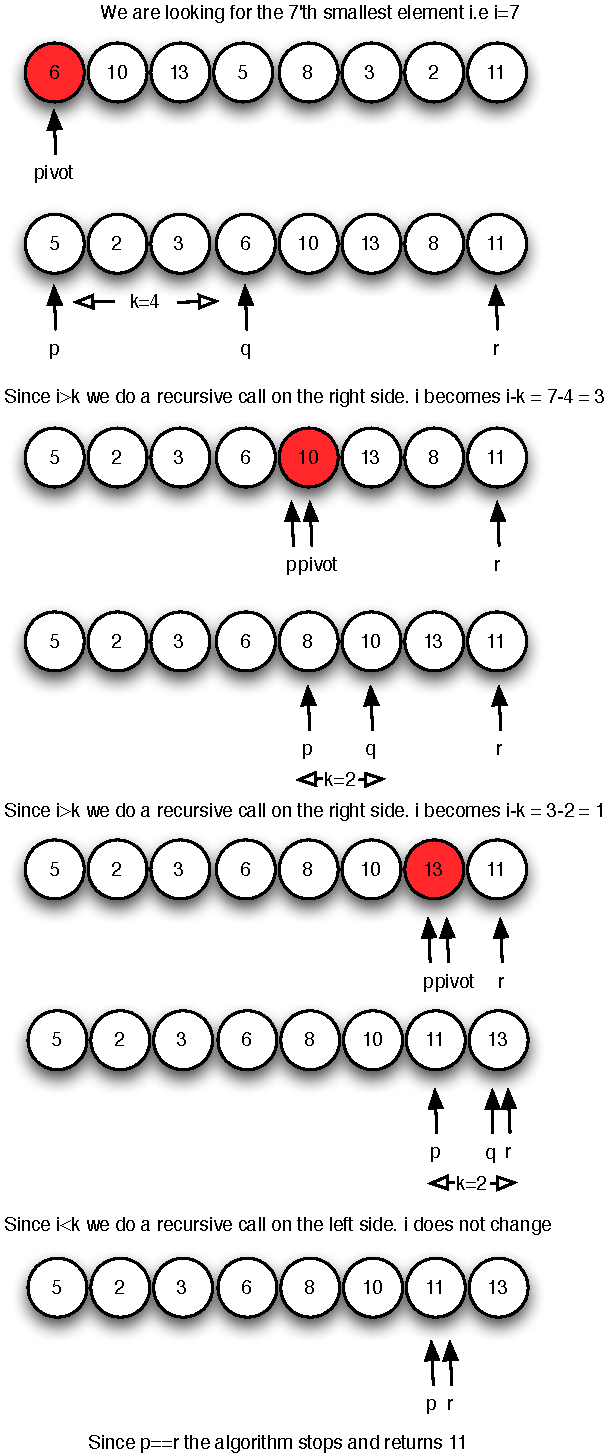
\includegraphics[width=0.6\textwidth]{figures/fig10.pdf}
\caption{Example run of the randomized select algorithm}
\label{fig10}
\end{figure}

% subsection selection_algorithm (end)


% section randomized_algoritms (end)

\clearpage \newpage
\section{Computational Geometry, Convex hulls} % (fold)
\label{sec:computational_geometry_convex_hulls}

\subsection{Disposition Computational Geometry, Convex hulls} % (fold)
\label{sub:disposition7}
\begin{itemize}
  \item What is a convex hull
  \item Grahams scan. Sorting $\O(n\log(n))$ + scanning of edges $\O(n)$. Total $\O(n\log(n))$
  \item Jarvis' march. Scanning takes $n$, and we need to scan $h$ times thus total is $\O(nh) = \O(n^2)$
  \item Chan - Uses both Grahams scan and Jarvis' march. Output sensitive $\O(n\log(h))$.
  \begin{itemize}
    \item Graham: $\O((n/h)h\log(h)) = O(n\log(h))$
    \item Jarvis' march: We can find the right tangent line between $p$ and any subhull in $O(\log(h))$ time using a variant of binary search. Since there are $n/h$ subhulls, finding the successor of $p$ takes $\O((n/h)\log(h))$ time together. Since there are $h$ convex hull edges, and we find each edge in $\O((n/h)\log(h))$ time, the overall running time of the algorithm is $\O(n\log(h))$.                                                                                                                                         
  \end{itemize}
  \item MBC <- if time permits
\end{itemize}

% subsection disposition7 (end)
\newpage 

Given a set of points $P$, the convex hull problem seeks to find a convex set containing all the points in $P$.

Let $S$ be a convex set. Then for any two points $a,b \in S$ the following is true
\begin{equation}
  (t-1)a+tb \qquad t \in [0,1]
\end{equation}
thus, there exists a line between any two points in $S$, such that the line between them is contained within $S$.

In the following we assume that no points has the same $x$- or $y$- coordinates and no three points are collinear. This is true in the continuous world, but watch out when going into the discrete world of computers!

We denote the convex hull of a set $S$ to be $CH(S)$. There exists several algorithms to calculate the convex hull. Int he following, Grahams scan, Jarvis' march, Quickhull, randomized incremental and marriage before conquest is explained in detail.

\subsection{Grahams scan} % (fold)
\label{sub:grahams_scan}
Grahams scan has a running time of $\O(n\log(n))$. It starts by choosing a the point $p_0 \in S$, with the lowest $y$-coordinate. This can be done in $\O(n)$. It then sorts the remaining points $p_i \in S$ by the angle between the line $(p_0, p_i)$ and the $x$-axis. This sorting can be done in $n \log(n)$ by e.g. heap sort\footnote{Heap sort uses a heap, i.e. a tree data structure where the largest element is on top.} 

Put $p_0, p_1, p_2$ in the list of nodes that constitutes the convex hull. If making a left turn when adding $p_3$, remove $p_2$ and add $p_3$ to the list. Otherwise if making a right turn, add $p_3$ to the list. Continue adding nodes. In general, if adding node $p_j$ creates a left turn, then remove node $p_{j-1}$ and add $p_j$. Otherwise just add $p_j$. When last node has been reached, the convex hull is done.

The correctness of Grahams scan can be explained by the following observations. 

\begin{itemize}
  \item Grahams scan will never go backwards behind the initial node. 
  \item When arriving at point $p_i$ all points between the initial node and the point $p_i$ are right turns on the polygonal line constructed so far
  \item After arriving at the initial node by a right turn, we get a polygonal line consisting of purely right turns. 
\end{itemize}

Figure \ref{fig16} shows an example run of Grahams scan.

\begin{figure}[ht]
\centering
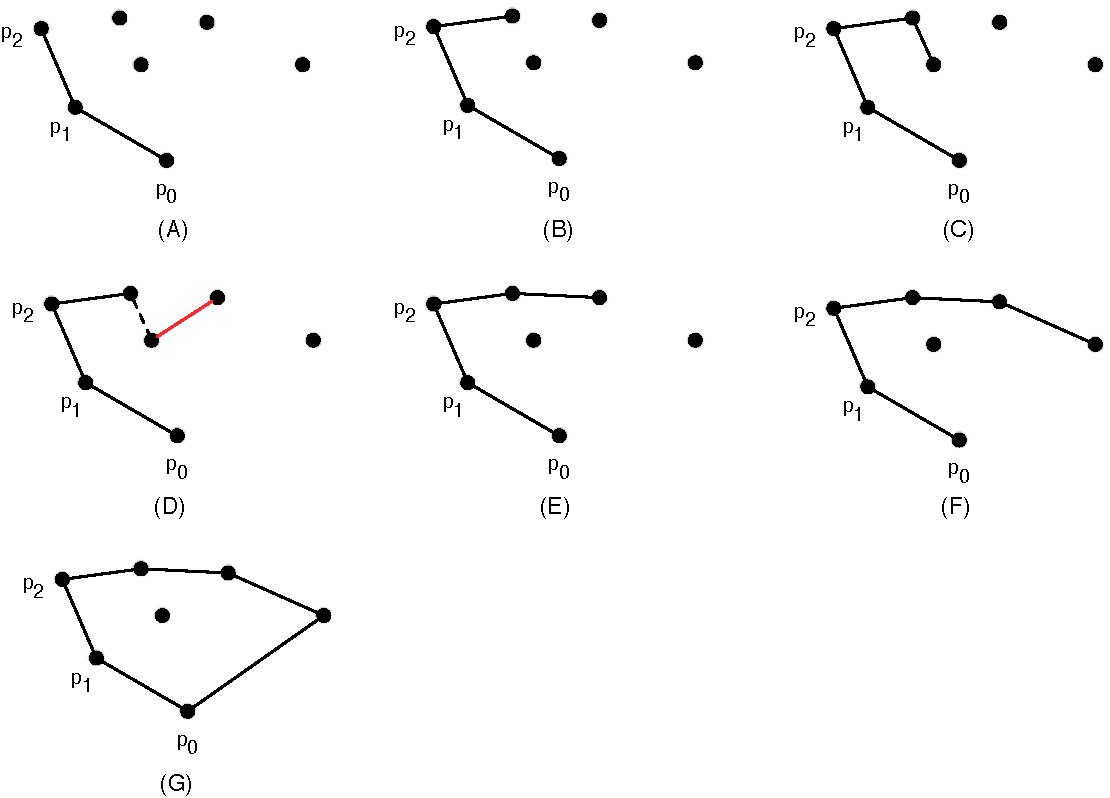
\includegraphics[width=0.75\textwidth]{figures/fig16.pdf}
\caption{Example run of Grahams scan}
\label{fig16}
\end{figure}

The time complexity is $\O(n\log(n))$ since sorting takes $\O(n\log(n))$ and the scanning takes $\O(n)$, since each point is only considered once. The total time complexity is thus $\O(n\log(n)+n)=\O(n\log(n))$.

% subsection grahams_scan (end)

\subsection{Jarvis' march} % (fold)
\label{sub:jarvis_march}
Jarvis' march is also knows as the `Gift wrapping algorithm'. It has a complexity of $\O(nh)$, where $n$ is the number of nodes, and $h$ is the number of nodes in the convex hull. Since part of the complexity relies on the final output, the algorithm is \emph{output sensitive} and can be $\O(n^2)$ when $h=n$.

Find the point, $p_0$, which is placed leftmost. This point can be found in $\O(n)$. Add $p_o$ to the convex hull list. Now find the point $p_1$ which has every other point $p_i$ to the right and add it to the list of convex hull nodes. This can also be done in $\O(n)$ by comparing polar angles from $p_0$. Continue to add $p_i$ to the list such that every other node is to the right of $p_i$. Continue until the $p_i=p_0$.

The complexity of Jarvis' march can be computed as the time it takes to find $p_i$ times the number of nodes, $h$ in the convex hull. The complexity is thus $\O(nh)$.

An example run of Jarvis' march can be seen on figure \ref{fig17}

\begin{figure}[ht]
\centering
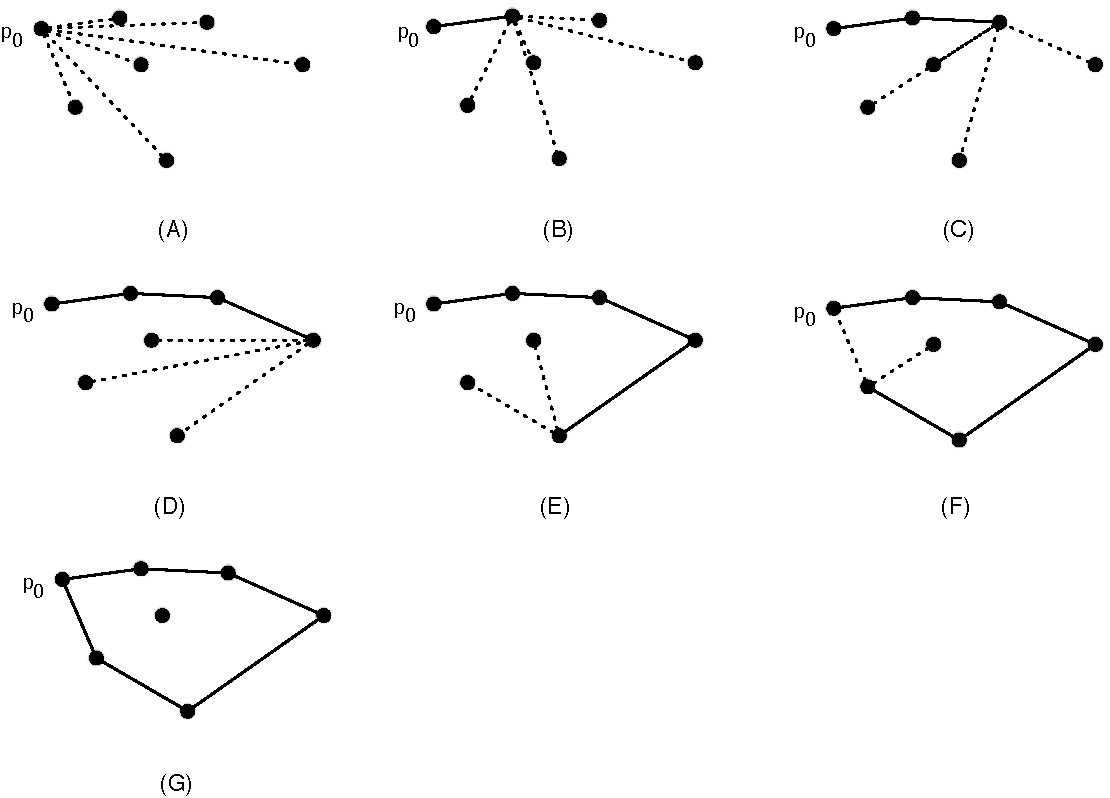
\includegraphics[width=0.75\textwidth]{figures/fig17.pdf}
\caption{Example run of Jarvis' march. The dotted lines are the polar angles}
\label{fig17}
\end{figure}


% subsection jarvis_march (end)


\subsection{Quickhull} % (fold)
\label{sub:quickhull}
Quickhull is an algorithm that has an expected running time of $\O(n\log(n))$, and a worst case running time of $\O(n^2)$. The algorithm starts by finding the leftmost and rightmost points, $A$ and $B$. It then draws a line between these two points, and splits the point set $S$ into two. Let the set $S_1$ contain the points above the line, and $S_2$ contain the points below the line. 

For each of these two sets we proceed recursively.

Find the point, $P$ farthest away from the line. the convex hull must contain $P$, so insert the point between $A$ and $B$. A triangle is formed by $ABP$. Remove all points from $S$ that is contained within this triangle. The cross product can be used to calculate wether a point lies inside a triangle.                                                                                        

We form two new sets. One set containing the set of points above the line $AP$. The other set containing points above the line $BP$. The line $AB$ is then replaced by these two lines. and the algorithm proceeds recursively. The algorithm stops when the sets are empty or if it only consist of one node.

An example run of Quickhull can be seen on figure \ref{fig18} 

\begin{figure}[ht]
\centering
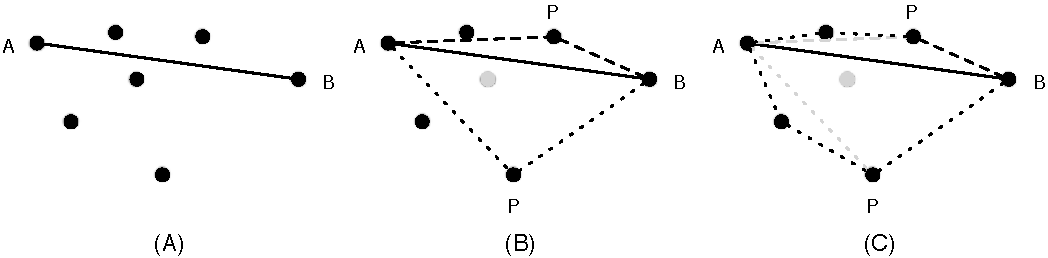
\includegraphics[width=0.75\textwidth]{figures/fig18.pdf}
\caption{Example run of quickhull. (A) find the left and right most points. (B) Recursively process the two subsets and find the point farthest away form the line. (C) Repeat recursively}
\label{fig18}
\end{figure}


If the partitioning yields balanced sets, the the expected running time is $\O(n\log(n))$. If the partitioning is extremely unbalanced then the running time is $\O(n^2)$. A example of an extremely unbalanced set of points, is when the points lie on a half circle.



% subsection quickhull (end)

\subsection{Marriage before conquest (MBC)} % (fold)
\label{sub:marriage_before_conquest_mbc_}
The Kirkpatrick-Seidel algorithm (Marriage before conquest) is output sensitive and has running time $\O(n\log{h})$, where $h$ is the number of points in the convex hull.

The algorithm first calculates the upper hull and then the lower hull. It then merges these two into the final convex hull. We can safely assume that the merging of the two half hulls can be performed in $\O(1)$.

\begin{itemize}
  \item Let $S$ be the set of points. Divide $S$ into two sets, by dividing $S$ with the line $(p_j,p_k)$, where $p_j \in S$ is the point with minimum $x$-value and $p_k \in S$ is the point with maximum $x$-value. Let $P$ be one of the two sets.                                                                                                                                        
  \item The algorithm then calculates the median $x$-coordinate $M$ of the points in $P$. It the finds the bridge segment that crosses the vertical line $x=M$. It finds this bridge segment by a technique called Prune \& Search. $x=M$ divides $P$ in half. The bridge segment across this line, will be part of the final convex hull. 
  \item Delete the points under the bridge, and split $P$ into the two half's divided by the vertical line. 
  \item Continue recursively on each half.
\end{itemize}


The Prune \& Search method works in the following way

\begin{itemize}
  \item Randomly pair all the points into line segments.
  \item Determine the median slope, $m$, of all the distinct line segments. If the number of points is odd, there will be a point that is not part of a line segment. Give this point a slope of $0$. If the number of line segments is even there are two choices for the median slope. Let $m$ be the max of these two slopes.
  \item Construct a sweep line, $L$, having the median slope, i.e $y = mx+b$. Find a point $p_t$ such that $L$ is a supporting line\footnote{A supporting line for a set $S$ is a line that contains a point $p_i \in S$ an no other points above.} for $P$ at $p_t$, this can be done by translating. We call $p_t$ the top point. 
  \item Let $p_j.x$ define the $x$-coordinate of the point $p_j$. 
  \begin{itemize}
    \item If $p_t.x \geq M$, i.e the top point is to the right of the vertical line M, then for each line segment with slope $< m$ remove the right point of the line segment, i.e $q_{ir}$.
    \item If $p_t.x < M$, i.e. the top point is to the left of the vertical line $M$, then for each line segment with slope $>m$, remove the left point $q_{il}$.
  \end{itemize}
  \item Repeat this until only two points are left. We know that at least half of the line segments has a slope greater than $m$, therefore we can conclude that we at each iteration of the bridge finding removes $1/4$ of the points. Note that the points are only removed in the current step where we find the bridge, not the set $P$.
\end{itemize}

Figure \ref{fig19} shows how to fine the bridge

\begin{figure}[ht]
\centering
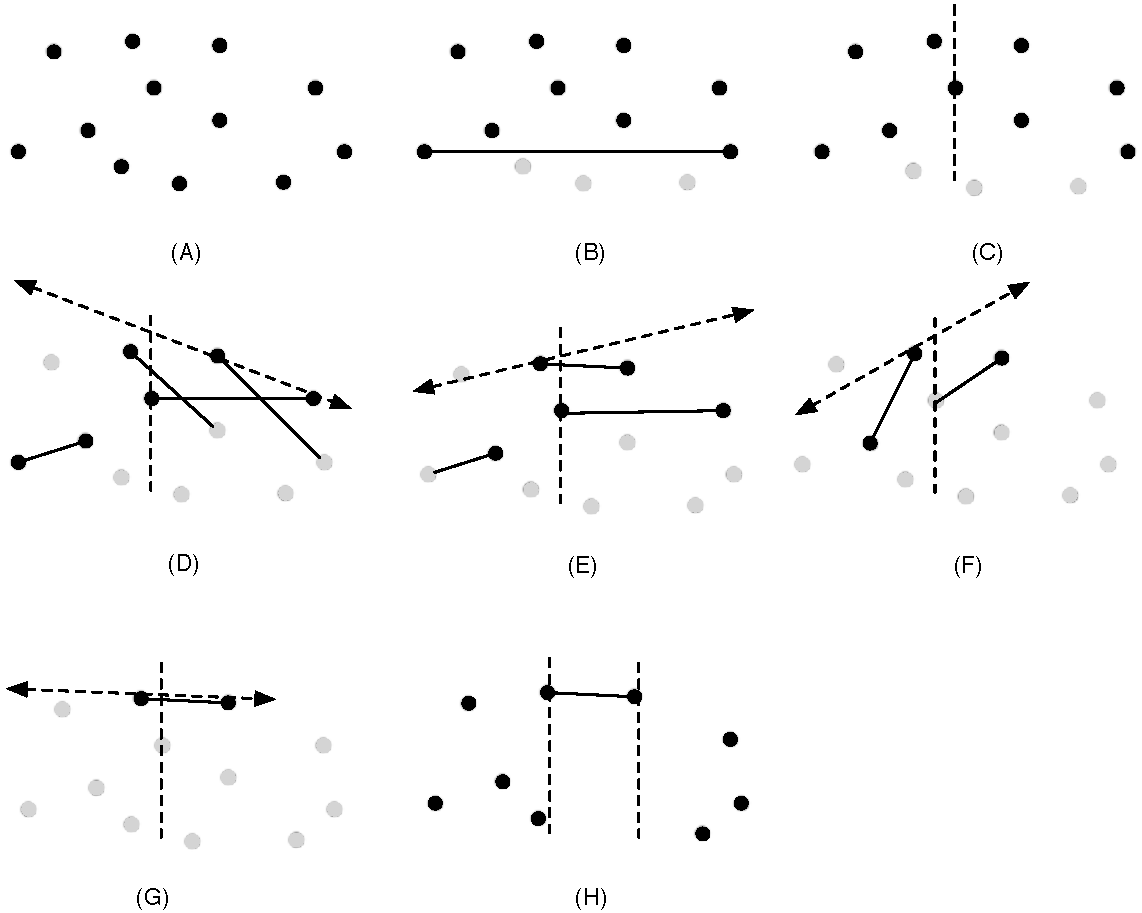
\includegraphics[width=0.9\textwidth]{figures/fig19.pdf}
\caption{(A) Original point set. (B) Separating the set in two. (C) Finding the median. (D) Pairing points, finding support line and removing points (grey color points are deleted). (E) Removing points. (F) Removing points. (G) Bridge found. (H) Deleting points under bridge}
\label{fig19}
\end{figure}

The complexity of the bridge finding is as follows. Pairwise point matching takes $\O(n)$, finding the median slope takes $\O(n)$, slope translation takes $\O(n)$. Each time we remove points we are sure to remove $1/4$ of the points. This yields 
\begin{align*}
T(n) &= \O(1) &\qquad n=2\\ 
T(n) &= T(3n/4) + \O(n) &\qquad \text{if } n>2
\end{align*}
thus the complexity of the bridge finding and finding the median is $T(n)=\O(n)$.

The total overall complexity can be bounded by the following function
\begin{align*}
f(n,h) &= cn &\qquad h=2  \\ 
f(n,h) &= cn + \max_{h_l+h_r = h}\left\{f(n/2,h_l)+f(n/2,h_r)\right\} &\qquad h>2
\end{align*}
where $c$ is a positive constant. The max is introduced because the algorithm is output sensitive. The claim is that the complexity is $f(n,h) = \O(n\log(h))$, thus we can find a upper bound by the function $cn\log(h)$.

\begin{proof}

  For $h=2$                
  \begin{equation}
    f(n,h) = c_1n \leq cn\log(2)
  \end{equation}
  this trivially holds if $c_1 \leq c$
  
  Assume $h>2$ and by substitution we have
  \begin{align*}
   f(n,h) &= cn + \max_{h_l+h_r = h}\left\{cn/2\log(h_l)+cn/2\log(h_r)\right\} \\
          &= cn + cn/2\max_{h_l+h_r = h}\left\{\log(h_l)+\log(h_r)\right\} \\
          &= cn + cn/2\max_{h_l+h_r = h}\left\{\log(h_lh_r)\right\} \\          
          &= cn + cn/2\max_{h_l+h_r = h}\left\{\log(h_l(h-h_l))\right\} \\         
          &= cn + cn/2\max_{h_l+h_r = h}\left\{\log(hh_l-h_l^2))\right\}                    
  \end{align*}
    
  When does the function $g(h_l) = \log(hh_l-h_l^2)$ takes it's maximum. It does when the derivative is $0$.
  \begin{equation}
    g_{h_l}'(h_l,h) = \frac{1}{hh_l-h_l^2} (h-2h_l) = 0 
  \end{equation}
  If $g_{h_l}'(h_l)=0$ then $h-2h_l=0$ yielding $h_l = \frac{h}{2}$. Thus
  \begin{align*}
   f(n,h) &= cn + cn/2\log(h\frac{h}{2}-\frac{h^2}{2^2})) \\
          &= cn + cn/2\log(\frac{h^2}{2}-\frac{h^2}{2^2})) \\   
          &= cn + cn/2\log(\frac{2h^2}{4}-\frac{h^2}{2^2})) \\
          &= cn + cn/2\log(\frac{h^2}{2^2})) \\                       
          &= cn + 2cn/2\log(\frac{h}{2}) \\                                 
          &= cn + cn\log(\frac{h}{2})                                 
  \end{align*}
   which has a running time of $\O(n\log(h))$
   
\end{proof}

% subsection marriage_before_conquest_mbc_ (end)


\subsection{Chan} % (fold)
\label{sub:chan_and_relations_to_mbc}
Chan is an algorithm that combines Grahams scan and Jarvis' march (gift wrapping). It is interesting because it involves combining two slower algorithms together to form an algorithm that is faster than either one.

The problem with Graham's scan is that it sorts all the points, and hence is doomed to having an $\O(n\log(n))$ running time, irrespective of the size of the hull. On the other hand, Jarvis's march can perform better if you have few vertices on the hull, but it takes $\O(n)$ time for each vertex in the hull.

The algorithm works as follows: 

\begin{itemize}
  \item First suppose we know there are $h$ points on the convex hull, this algorithm starts by shattering the input points in $n/h$ arbitrary subsets, each of size $h$, and computing the convex hull of each subset using Graham's scan. This much of the algorithm requires $\O((n/h)h\log(h)) = O(n\log(h))$ time.
  \item Once we have the $n/h$ subhulls, we follow the general outline of Javis's march, wrapping a string around the $n/h$ subhulls. Start with the leftmost input point $l$, starting with $p = l$ we successively find the convex hull vertexes in counter-clockwise order until we return back to the original leftmost point again.
  \item The successor of $p$ must lie on a right tangent line between $p$ and one of the subhulls, a line from $p$ through a vertex of the subhull, such that the subhull lies completely on the right side of the line from $p$'s point of view. We can find the right tangent line between $p$ and any subhull in $O(\log(h))$ time using a variant of binary search. Since there are $n/h$ subhulls, finding the successor of $p$ takes $\O((n/h)\log(h))$ time together. Since there are $h$ convex hull edges, and we find each edge in $\O((n/h)\log(h))$ time, the overall running time of the algorithm is $\O(n\log(h))$.
\end{itemize}

An example run can be seen in figure \ref{fig22}.


\begin{figure}[ht]
\centering
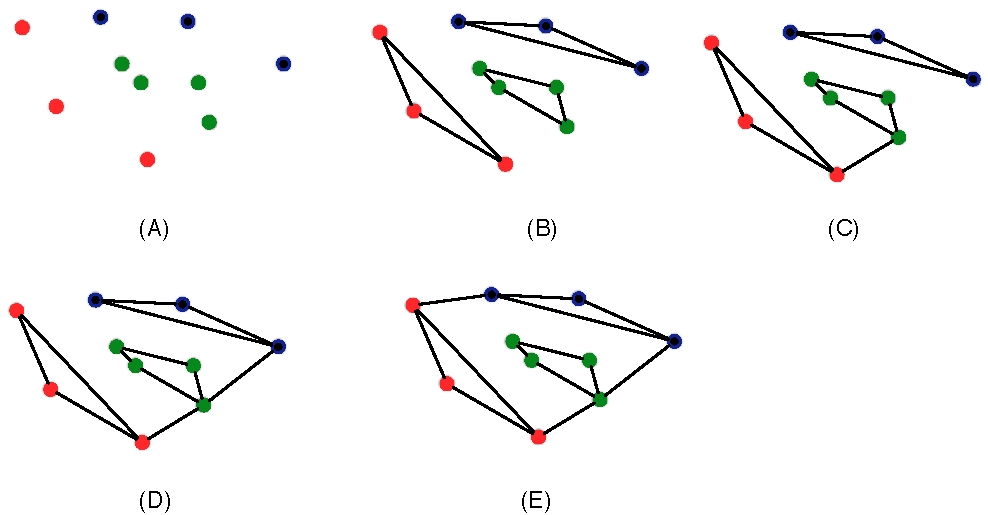
\includegraphics[width=0.75\textwidth]{figures/fig22.pdf}
\caption{Example run of the Chan algorithm.}
\label{fig22}
\end{figure}

Unfortunately, this algorithm only takes $O(n\log(h))$ time if we know the value of $h$ in advance. So how do we know $h$'s value? Chan's trick is to guess the correct value of $h$, let's denote the guess by $h'$. Then we shatter the points into $n/h'$ subsets of size $h'$, compute their subhulls, and then find the first $h'$ edges of the global hull. If $h < h'$, this algorithm computes the complete convex hull in $O(n\log(h'))$ time. Otherwise, the hull doesn't wrap all the way back around to $l$, so we know our guess $h'$ is too small.

Chan's algorithm starts with the optimistic guess $h' = 3$. If we finish an iteration of the algorithm and find that $h'$ is too small, we square $h'$ and try again. In the final iteration, $h'<h^2$, so the last iteration takes $\O(n\log(h')) = \O(n\log(h^2)) = \O(n\log(h))$ time.

The total running time of Chan's algorithm is given by the sum: $\O(n\log(3) + n\log(3^2) + n\log(3^4) + ... + n\log(3^{2^k}))$ , for some integer $k$. We can rewrite this as a geometric series: $\O(n\log(3) + 2n\log(3) + 4n\log(3) + ... + 2kn\log(3))$. So Chan's algorithm runs in $\O(n\log(h))$ time overall, even when we don't know the value of $h$.


% subsection chan_and_relations_to_mbc (end)

% section computational_geometry_convex_hulls (end)

\clearpage \newpage
\section{Computational Geometry, Delaunay triangulation} % (fold)
\label{sec:computational_geometry_delaunay_triangulatiom}

\subsection{Disposition Computational Geometry, Delaunay triangulation} % (fold)
\label{sub:disposition8}
\begin{itemize}
  \item Applications
  \item Good triangulation - edge flip
  \item Naive method - add edges without crossing already made edges
  \item Example of Delaunay, big triangle, maintenance of point location data structure
  \item Voronoi diagram from circumcircle 
\end{itemize}
\newpage
% subsection disposition (end)

\subsection{Applications} % (fold)
\label{sub:applications}
Triangulation is used in graphics and movies. It can also be used to model terrain when the terrain is represented as a bunch of sample points where each sample point is representing the height of the terrain compared to, lets say, sea level. A terrain visualized solely by height samples is not that interesting an doesn't look very natural! Instead we can do triangulation of the samples in 2D, and after the triangulation lift the points op in 3D yielding a triangulated surface, representing a terrain. 

The central question here is how we triangulate the points? and if there are multiple methods how do we choose the method that gives us the most appropriate triangle net? In the following subsections we will answer these two questions.
% subsection applications (end)applications


\subsection{Definition} % (fold)
\label{sub:definition}

What do we mean by a good triangulation?
Simple case is to connect one point to every other point. This is NOT a good triangulation. The ideal triangulation is a triangulation that is balanced, i.e. the we want to avoid small angles. 

We define angle optimality as follows.

Let $T$ be a triangulation of $P$. Let $T$ consist of $m$ triangles. Then $T$ has $3m$ angles. Let the angles be in a sorted vector in increasing order. Denote this vector $A(T)$ We call this vector an \emph{angle vector}. Let $T'$ be another triangulation of $P$. We say that $T$ is \emph{angel-optimal} if $T$ is lexicographically larger than $\forall T'\in P$.

Lexicographically larger means that for some index $i$ the angles after $i$ in $A(T)$ is larger than the angels in $A(T')$. E.g.

\begin{equation} 
\left(
\begin{array}{r} 
   1  \\
   3 \\
   5 \\
   7 
\end{array} 
\right) >   
\left(
\begin{array}{r} 
   1  \\
   2 \\
   5 \\
   7 
\end{array} 
\right)
\end{equation} 
the reason for this definition, is we want as uniform angles as possible in all triangles.


We define maximal planar subdivision as
\begin{definition}
Maximal planar subdivision: A subdivision $S$ such that no edge connecting two vertices can be added to $S$ without destroying it's planarity, i.e. any edge not in $S$ intersects and edge $e \in S$.  
\end{definition}
from the maximal planar subdivision we can define the triangulation as
\begin{definition}
Triangulation of set of points $P$: A maximal planar subdivision whose vertices are elements of $P$.  
\end{definition}

% subsection definition (end)



\subsection{Edge flip} % (fold)
\label{sub:edge_flip}
Given two adjacent triangles $p_1 p_2 p_4$ and $p_2 p_3 p_4$, one can do an edge flip as follows. Remove the common edge by creating two new triangles consisting of $p_1 p_3 p_4$ and $p_1 p_2 p_3$. An illustration of an edge flip can be seen on figure \ref{fig6}.

In the two adjacent triangles there are 6 angles. If we can increase the minimum angle by doing a edge flip on the shared edge, we called the shared edge illegal.

\begin{figure}[ht]
\centering
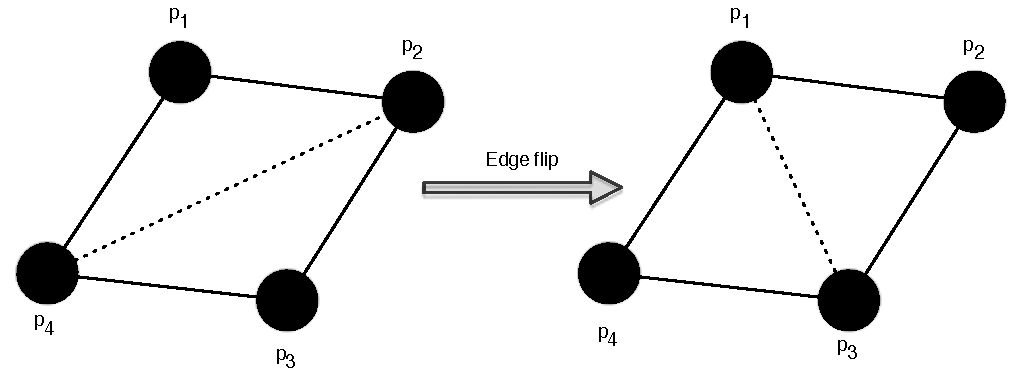
\includegraphics[width=0.8\textwidth]{figures/fig6.pdf}
\caption{Example of an edge flip}
\label{fig6}
\end{figure}

Instead of checking wether an edge is illegal by computing all the angles, we can use the following observation

\begin{figure}[ht]
\centering
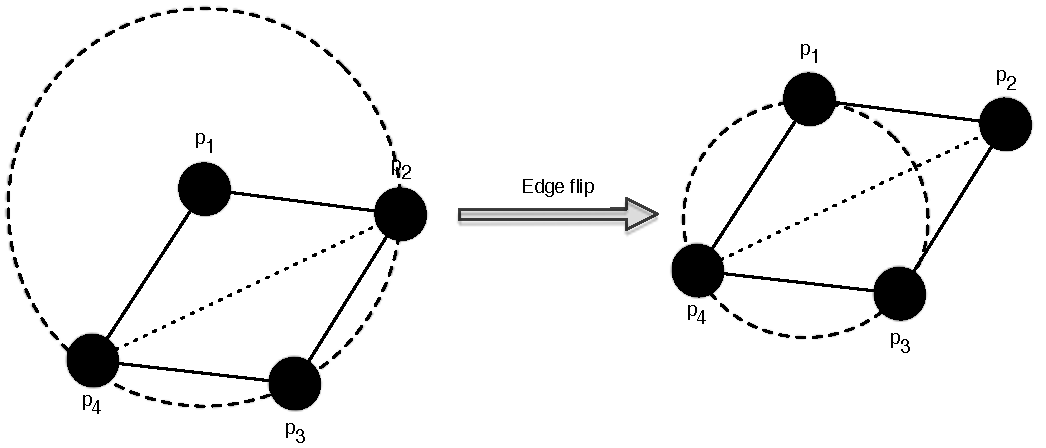
\includegraphics[width=0.9\textwidth]{figures/fig7.pdf}
\caption{If $p_1$ is inside the circumcircle then the edge between the two triangles is illegal an we perform an edge flip.}
\label{fig7}
\end{figure}
% subsection edge_flip (end)


\subsection{Delaunay triangulation} % (fold)
\label{sub:delaunay_triangulation}
The Delaunay triangulation for a set of points $P$ is a triangulation where no point $p_i \in P$ is inside the circumcircle of any triangle in the triangulation set. The Delaunay triangulation is actually the dual of the Voronoi diagram. figure \ref{fig8} shows this relation. 

The Voronoi diagram is shown as red on figure \ref{fig8}, while the triangulation is shown as black. A line in the Voronoi diagram separating two vertices, indicates that there is an edge between the two vertices in the triangulation.

\begin{figure}[ht]
\centering
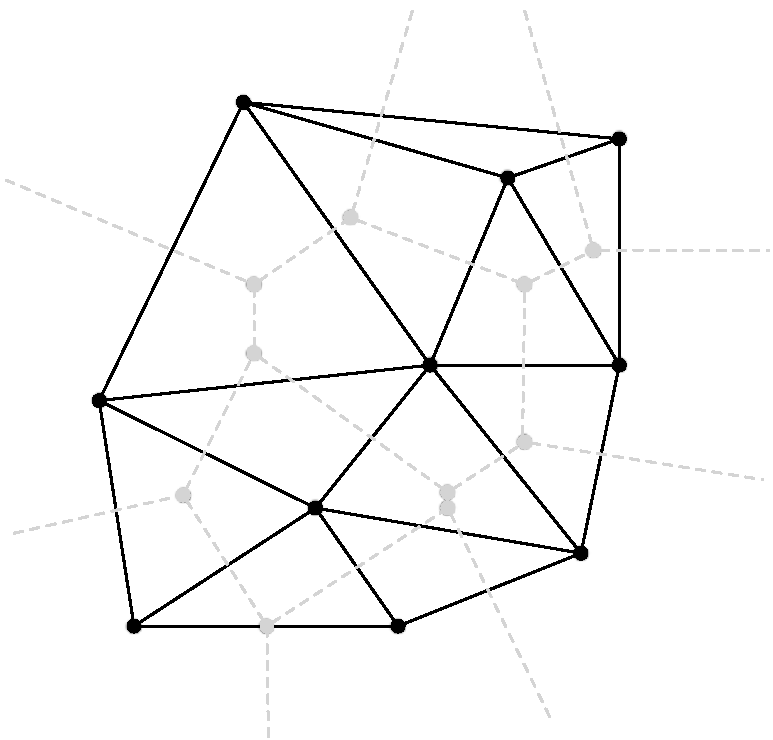
\includegraphics[width=0.7\textwidth]{figures/fig8.pdf}
\caption{Duality between the Delaunay triangulation and the Voronoi diagram.}
\label{fig8}
\end{figure}

Returning to the legal and illegal edges. Let $P$ be a set of points in the plane then a triangulation of $P$ is legal, \emph{if and only if}, the triangulation is a Delaunay triangulation.
% subsection delaunay_triangulation (end)


\subsection{Naive method} % (fold)
\label{sub:naive_method}
Given a set of points, \emph{take the convex hull}, add diagonals (edges that connects vertices), without crossing those we already have drawn, until there are no more vertices. The result is a triangulation. I.e. we partition the points into triangles.

In order to make the triangulation into a Delaunay triangulation, we can do edge flips until there are no more illegal edges.


The most straightforward way of efficiently computing the Delaunay triangulation is to repeatedly add one vertex at a time, re-triangulating the affected parts of the graph. When a vertex v is added, we split in three the triangle that contains v, then we apply the flip algorithm. Done naively, this will take O(n) time: we search through all the triangles to find the one that contains v, then we potentially flip away every triangle. Then the overall runtime is O(n2).

% subsection naive_method (end)


\subsection{Computing the Delaunay triangulation} % (fold)
\label{sub:computing_the_delaunay_triangulation}
The algorithm is randomized incremental algorithm, adding one point at a time.

Let $P$ be the set of points we want to triangulate. Find the point with the highest $y$ coordinate, and name this point $p_0$. Make a big triangle, that contains all the points in $P$ such that $p_0$ is one of the corners in the triangle. 

Now pick a random point from $P$ and add it to the big triangle, such that the big triangle is divided into $3$ sub triangles. Run a legalize edge procedure, ensuring that all the edges are legalized.

Keep adding points from the set $P$, and legalize the edges of until $P$ is empty. 

As a final stage remove the points $p_{-1}$ and $p_{-2}$ along with the incident edges. 

THe data structure used is a point location structure. It is a tree like structure where the nodes defines the position of previous triangles and the leafs corresponding to the current visible triangles. 

Given a point the data structure makes it possible to locate the triangle of which the point is placed upon. 

Figure \ref{fig9} shows how the data structure is maintained when splitting existing triangles and flipping edges.
\begin{figure}[ht]
\centering
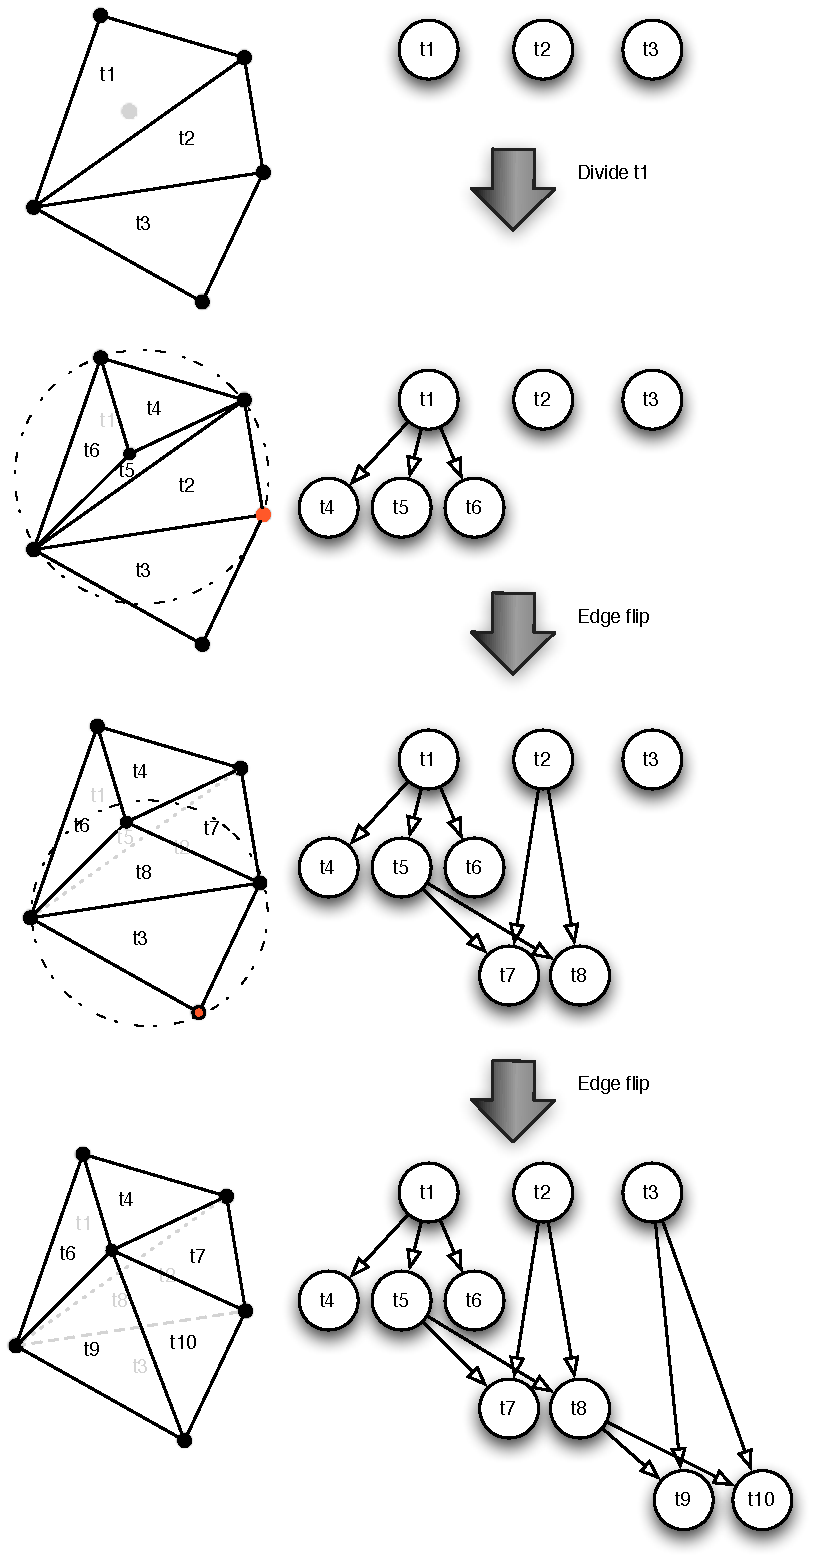
\includegraphics[width=0.75\textwidth]{figures/fig9.pdf}
\caption{Example of maintaining a data structure when flipping edges and dividing triangles.}
\label{fig9}
\end{figure}

The \emph{expected} running time of the algorithm is $\O(n\log(n))$. This can be explained as, it takes constant time to create new triangles the maximal number of triangles created is $\O(n)$. When identifying the triangle in which a point is located, we use the point location data structure, and can make this identification in $\O(\log(n))$.

% subsection computing_the_delaunay_triangulation (end)

\subsection{Voronoi diagram} % (fold)
\label{sub:voronoi_diagram}
The Voronoi diagram can be made by the Delaunay triangulation by calculating the circumcircles of every triangle in the Delaunay. The centers of the circumcircles are vertices in the Voronoi diagram. The centers can be connected by edges so the each edge is the shortest possible. 

\begin{figure}[ht]
\centering
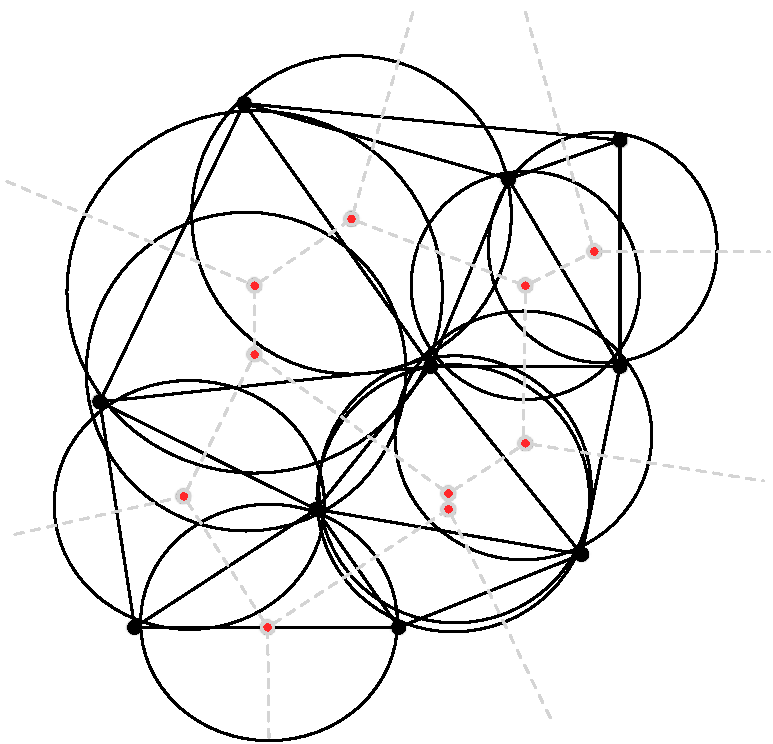
\includegraphics[width=0.9\textwidth]{figures/fig23.pdf}
\caption{Example of calculating the Voronoi diagram from the Delaunay triangulation}
\label{fig23}
\end{figure}


% subsection voronoi_diagram (end)

                                       
% section computational_geometry_delaunay_triangulatiom (end)


\end{document}